\documentclass[doc,biblatex]{apa7}
\usepackage{amsmath}
\DeclareLanguageMapping{american}{american-apa}
\addbibresource{references.bib}

\captionsetup[figure]{textfont=rm,font=footnotesize} % Override italic APA figure 
\captionsetup[table]{textfont=rm,font=footnotesize} % Make table captions smaller
\usepackage{chngpage} % to fit table centrally on page

% temp for revision %%%%%%%%%%%%%%%%%%%%%%%%%%%%
\usepackage{xcolor}
\newcommand\newmaterial[1]{\textcolor{blue}{#1}}
%%%%%%%%%%%%%%%%%%%%%%%%%%%%%%%%%%%%%%%%%%%%%%%%

\title{Readers target words where they expect to minimize uncertainty}

\shorttitle{Readers target words to minimize uncertainty}

\authorsnames[{1,2},1,1,1]{Jon W. Carr, Monica Fantini, Lorena Perrotti, Davide~Crepaldi}

\authorsaffiliations{{Cognitive Neuroscience, International School for Advanced Studies, Trieste, Italy},{Department of Psychology, Royal Holloway, University of London, England}}

\authornote{\textbf{Cite as:} Carr, J.\@ W., Fantini, M., Perrotti, L., \& Crepaldi, D.\@ (2024). Readers target words where they expect to minimize uncertainty. \textit{OSF Preprints}. Version~4. http://doi.org/10.31219/osf.io/r5n3g}

\abstract{Skilled readers use multiple heuristics to guide their eye movements during reading. One possible cue that readers may rely on is the way in which information about word identity is typically spread across words. In many (but not all) languages, words are, on average, more informative on the left, predicting that readers should have a preference for left-of-center fixation when targeting words. Any such effect will, however, be modulated by important perceptual constraints and may be masked by various confounding factors. In three experiments with artificially constructed lexicons, we provide causal evidence that the way in which a language distributes information affects how readers land on words. We further support our analyses with a Bayesian cognitive model of visual word recognition that predicts where readers ought to fixate in order to minimize uncertainty about word identity. Taken together, our findings suggest that global properties of the lexicon may play a role in isolated word targeting, and may therefore make a contribution to eye movement behavior in more natural reading settings.}

\keywords{eye movements; optimal viewing position; reading; statistical learning; visual word recognition}

\begin{document}

\maketitle

\noindent
Skilled readers are able to interpret a written text with remarkable ease and efficiency despite the fact that writing is a complex code that takes on a multitude of visual forms and reflects the many layers of complexity that are inherent to human language---from individual letters and how they combine to morphosyntactic structure and beyond. To make this possible, readers must learn reliable heuristics, rapidly combine multiple sources of information, and contend with a range of competing trade-offs \parencite{Rayner:1998, Yeatman:2021, Snowling:2022}.

One general cue that readers may rely on is the way in which information about word identity is typically spread across words within a given lexicon \parencite{Farid:1996, Clark:1999, Deutsch:1999, Alhama:2019, Shafir:2022}. In many---but not all---languages, the most informative content is, on average, concentrated closer to word onset. For example, the first three letters of \textit{guarded} are much more informative than the last three, since there are few words in English that begin with \textit{gua-} and many that end with \textit{-ded}. \newmaterial{A number of explanations have been put forward to explain why words might be more informative at their beginnings. The most obvious reason is because languages are---first and foremost---adapted for the efficient production and comprehension of speech; thus, there may be pressures acting on the language to position informative content earlier in words, allowing the so-called uniqueness point to be reached more rapidly \parencite{MarslenWilson:1987}. Another possibility relates to the cross-linguistic suffixing preference that has long been noted \parencite{Greenberg:1957}, perhaps due to processing or learning biases \parencite{Cutler:1985, Hawkins:1988, Martin:2020, Ramscar:2013, StClair:2009}.} But whatever the underlying origin, such structural asymmetries in the lexicon---the lexicon's ``informational bias''---may explain why readers identify words more accurately when fixating closer to word onset \parencite[the optimal viewing position;][]{ORegan:1984, Brysbaert:2005, Hyona:2011} and why readers prefer to target words closer to word onset during continuous reading \parencite[the preferred landing position;][]{McConkie:1988, Vitu:1990, Ducrot:2002}.

Nevertheless, evidence for a direct causal relationship between typical information spread and reading behavior is difficult to obtain for two principal reasons. First, during normal reading, a reader's decision about where to fixate a word may be influenced by several competing factors, including prior sentence context \parencite{Balota:1985}, preview of the upcoming word from the parafovea \parencite{Hyona:1989, Underwood:1990, Schotter:2011}, \newmaterial{saccade planning \parencite{Engbert:2010, Krugel:2014, McDonald:2004}}, and constraints on perception \parencite{Bouma:1973, McConkie:1975}. Of particular relevance is the finding that humans have an asymmetric visual span (typically a right-visual-field advantage), which has \newmaterial{primarily} been attributed to \newmaterial{two possible (and non-mutually exclusive) origins:} cerebral lateralization \newmaterial{making it easier to process linguistic content in the right visual field} \parencite{Brysbaert:1988, Bub:1988, Ellis:2004, VanderHaegen:2013} and/or learned reading habits \newmaterial{relating to reading direction} \parencite{Huey:1900, Mishkin:1952, Pollatsek:1981}. We take a neutral stance on this debate, referring to any such asymmetry as the reader's ``perceptual bias,'' \newmaterial{which we construe broadly to include anything that the human reader brings to the table in the process of visual word recognition}. Importantly, this perceptual bias of the reader---like the informational bias of the lexicon, as described above---also typically predicts a preference for left-of-center fixation, making the two biases difficult to disentangle.

The second reason why it is difficult to test for a causal connection between the structure of the lexicon and reading behavior is that doing so necessitates the comparison of two or more natural languages. However, direct comparison of any two languages will be fraught with challenges because they will differ in many more ways than information distribution alone. For example, to date, the best available evidence has come from comparisons of languages written in left-to-right vs.\@ right-to-left scripts \parencite{Pollatsek:1981, Farid:1996, Deutsch:1999}. In a right-to-left script (e.g., Arabic or Hebrew), the informative linguistic content is typically located on the right, predicting a preference for right-of-center fixation, albeit modulated to some extent by the aforementioned perceptual factors \parencite{Nazir:2004, Brysbaert:2005}. However, comparison of languages written in different directions does not hold all factors constant. For example, the Arabic and Hebrew scripts are both abjads (scripts in which vowel sounds are represented by diacritics or, more commonly, not at all), which dramatically changes how much information is carried by each letter. Arabic is a cursive script, which may promote word decomposition at a higher level of analysis than individual letters \parencite{Farid:1996}. Hebrew has a complex, non-concatenative morphology, which may result in different mechanisms of word recognition \parencite{Velan:2011}. Readers of Arabic and Hebrew are also likely to have at least somewhat regular exposure to left-to-right reading due to the widespread use of the Latin script, especially among the types of people who typically take part in psychological experiments \parencite{Ducrot:2002, Sieroff:2015}.

These two sets of issues---the complex interplay of several factors that determine where a reader will fixate a word during ordinary reading, along with the many confounds inherent to comparing natural languages---have made it difficult to evaluate the longstanding claim that lexical constraint plays a role in fixation patterns, as hypothesized by \textcite[p.~298]{ORegan:1981}. Herein, we attempt to evaluate this claim by taking a rather different approach. Rather than compare reading behavior in natural languages, we construct two artificial lexicons---two idealized test cases---that are identical except for the way in which information is spread laterally across words, eliminating any possible linguistic confounds (e.g., differences in orthography, script direction, morphosyntactic structure, etc.). To support our analyses, we set out a formal model of visual word recognition that explicitly captures the perceptual bias (i.e., whatever the reader brings to the table) and informational bias (i.e., whatever the language brings to the table), allowing us to study the independent effects of perception and information, as well as their interaction. Ultimately, we show that the informational structure of the lexicon has a causal effect on how people identify and target words, and that this effect can be explained though a general computational principle of uncertainty minimization.

\section{Data Availability}

All data and code for the model, cross-linguistic analysis, and experiments are publicly accessible at \url{https://osf.io/s3gev/}

\section{Cognitive Model and Cross-Linguistic Analysis}

\begin{figure}
\makebox[\textwidth][c]{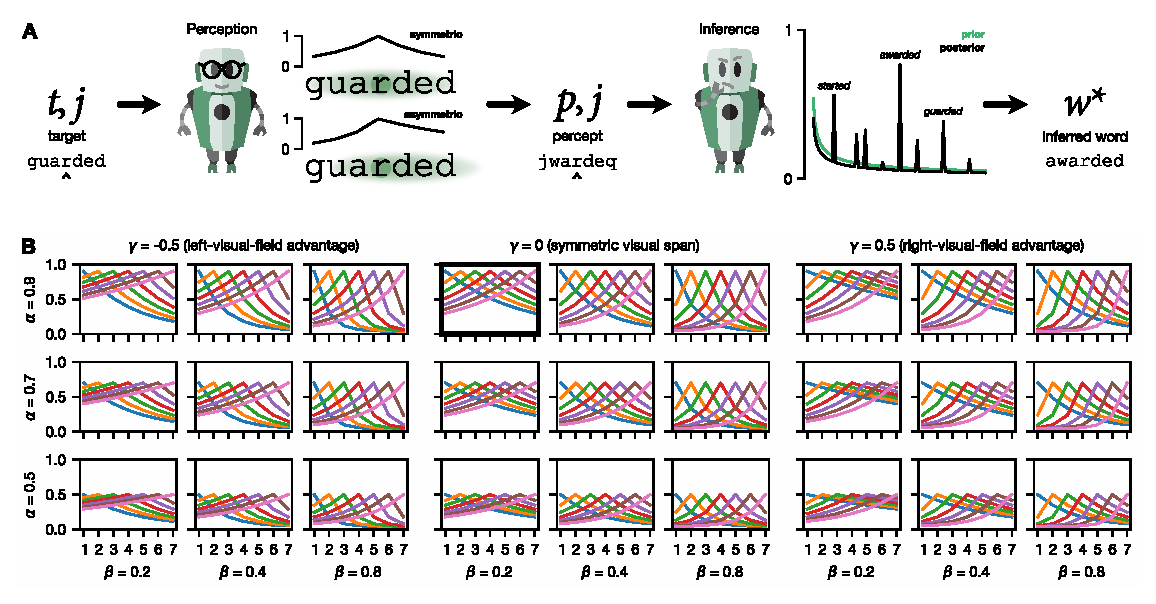
\includegraphics[]{figs/fig01.eps}}
\vspace*{2pt}
\caption{\textbf{A}~Illustration of a single trial in the core modeling framework. A target word $t$ is fixated in position $j$ and passes through the reader's perceptual filter, resulting in percept $p$. Given this percept, the reader makes an inference about the target word by updating its frequency-based prior in light of the perceptual evidence. In the example, the reader is exposed to \textit{guarded} in central position but incorrectly infers the word \textit{awarded}. \textbf{B}~Each panel represents the perceptual filter $\Phi(i|j)$ under a particular setting of $\alpha$, $\beta$, and $\gamma$ and shows the probability ($\Phi$; \textit{y}-axes) of correctly identifying the character in positions 1 through 7 ($i$; \textit{x}-axes) given a fixation in positions 1 though 7 ($j$; blue through pink). For example, if the parameters are set to $\alpha=0.9$, $\beta=0.2$, and $\gamma=0$ (the panel highlighted with a thicker frame) and the reader is fixating in central position ($j=4$; red curve), then the probability of correctly perceiving the characters in initial ($i=1$) or final ($i=7$) position is around 0.5.}
\label{fig01}
\end{figure}

We began by formulating a high-level Bayesian cognitive model of visual word recognition that explicitly encodes the perceptual and informational biases (Fig.~\ref{fig01}A). This model allowed us to explore how the two biases interact and understand how this interaction is likely to play out in natural languages. Furthermore, we used the model to aid in the interpretation of Experiment~1 and to help us make concrete predictions about Experiment~2.

\subsection{Method}

The model shares similarities with several other ``Bayesian reader'' models \parencite{Norris:2006, Norris:2009, SmithChan:2010, Bicknell:2012, Norris:2012, Valdois:2021}. The model conceptualizes visual word recognition as a simple two-stage process, comprised of perception and inference (see Fig.~\ref{fig01}). In the perception stage, the reader attempts to identify the letters in the word, forming a noisy percept. In the inference stage, the reader combines this perceptual evidence with prior information about what the word might plausibly be, forming a posterior over the lexicon from which it can choose a good candidate word.

\subsubsection{Model description}

The reader's lexicon $W$ consists of $n$ words of some constant length $m$, which are written using the set of symbols $S$. During perception, the constituent letters of a target word $t$ may be corrupted according to the function $\Phi$, which we refer to as the reader's ``perceptual filter.'' This function dictates the probability of correctly perceiving the letter in position $i$ given a fixation in position $j$, and is defined as follows:
\begin{equation}
\Phi(i|j) =
\begin{cases}
    (\alpha - \frac{1}{|S|}) \exp [ \beta (\gamma - 1) (i - j) ] + \frac{1}{|S|} & \text{if $i > j$} \\
    (\alpha - \frac{1}{|S|}) \exp [ \beta (\gamma + 1) (i - j) ] + \frac{1}{|S|} & \text{otherwise.}
\end{cases}
\label{eq_filter}
\end{equation}
\newmaterial{The use of the exponential function here results in the probability of successfully identifying a character gradually approaching chance with distance.} The perceptual filter, which is illustrated in Fig.~\ref{fig01}B, is controlled by three parameters:
\begin{itemize}
    \item $\alpha \in [\frac{1}{|S|}, 1)$ controls the probability that the reader will correctly identify the character under fixation within some fixed period of time (e.g., 50~ms).
    \item $\beta > 0$ controls the rate at which this probability approaches chance ($\frac{1}{|S|}$) with distance from the fixation position. Larger values result in a more rapid drop in probability and therefore a narrower visual span.
    \item $\gamma \in (-1, 1)$ controls the symmetry of the visual span. When $\gamma = 0$ the probability of correct letter identification drops symmetrically to the left and right (i.e., no perceptual bias). When $\gamma$ is positive, the reader is more likely to correctly perceive letters to the right of fixation compared to letters to the left (i.e., a right-visual-field advantage). The reverse is true when $\gamma$ is negative.
\end{itemize}
\newmaterial{If a character is perceived incorrectly (i.e., with probability $1 - \Phi(i|j)$), one of the other $|S|-1$ symbols will be perceived instead with uniform probability, $(1 - \Phi(i|j)) / (|S| - 1)$. This represents a simple model of perception that could be extended by, for example, taking letter confusability into account.}

At the inference stage, the reader combines its noisy perceptual evidence with prior information about word frequency, forming a posterior over the lexicon. Given a percept $p$ and knowledge of the fixation position $j$, the posterior probability of a hypothesized word $w$ is given by Bayes' rule: $\mathrm{Pr}(w|p,j) \propto \mathrm{Pr}(p|w,j) \mathrm{Pr}(w)$. The likelihood term, $\mathrm{Pr}(p|w,j)$, denotes the probability that the perceptual filter would have given rise to percept $p$ given that the true target was $w$ fixated in position $j$. Following the definition of perception outlined above, the likelihood is therefore given by
\begin{equation}
\mathrm{Pr}(p|w,j) = \prod_{i=1}^m
\begin{cases}
       \Phi(i|j)                   & \text{if $p(i) = w(i)$} \\
       \frac{1 - \Phi(i|j)}{|S|-1} & \text{otherwise,}
\end{cases}
\label{likelihood}
\end{equation}
where $p(i)$ and $w(i)$ represent the $i$th characters of $p$ and $w$. The prior term, $\mathrm{Pr}(w)$, denotes the probability of a hypothesized word being true before the observation of any perceptual evidence and is set to the relative frequency of the word:
\begin{equation}
\mathrm{Pr}(w) = \frac{\mathrm{F}(w)}{\sum_{w^\prime \in W} \mathrm{F}(w^\prime)}.
\label{prior}
\end{equation}
\newmaterial{This represents a simple assumption about the prior information available to the reader in the case of isolated word reading, but the model could be extended here by incorporating prior information from sentence context or parafoveal preview}. Finally, the model reader infers word $w^\ast = \mathrm{arg\,max}_{w \in W} \mathrm{Pr}(w|p,j)$, the word with maximum posterior probability.

\subsubsection{Measure of uncertainty}

During a single instance of visual word recognition, the uncertainty experienced by the reader may be quantified as the entropy of its posterior:
\begin{equation}
\mathrm{H}(W|p,j) = -\sum_{w \in W} \mathrm{Pr}(w|p,j) \log [\mathrm{Pr}(w|p,j)].
\label{entropy}
\end{equation}
If the reader's posterior tends to concentrate much of the probability mass on a single word, then uncertainty will be low; in contrast, if the reader's posterior distributes the probability mass fairly equally across a variety of words, uncertainty will be high. The expectation of this quantity---that is, averaging over all words the reader might encounter and all percepts that might be formed in response to those words---may then be defined as follows:
\begin{equation}
\mathrm{U}(j) = \sum_{t \in W} \sum_{p \in P} \mathrm{Pr}(t) \mathrm{Pr}(p|t,j) \mathrm{H}(W|p,j).
\label{uncertainty}
\end{equation}
In other words, we define the level of uncertainty a reader can expect to experience when fixating in position $j$ as average posterior entropy,\footnote{Since Equation~\ref{uncertainty} is intractable for even modest symbol sets and word lengths (i.e., because the number of possible percepts $|P| = |S|^m$), we estimate its value by simulating some large number of reading events.} weighted by the probability of a particular target word occurring \newmaterial{($\mathrm{Pr}(t)$; Equation~\ref{prior})} and the probability of a particular percept being formed given that target \newmaterial{($\mathrm{Pr}(p|t,j)$; Equation~\ref{likelihood})}. The letter position that, on average, minimizes uncertainty is thus given by $\mathrm{arg\,min}_{j=1}^m \mathrm{U}(j)$. Our contention is that human readers develop implicit knowledge of the position that minimizes uncertainty (i.e., taking into account both the statistical structure of the lexicon and the reader's own perceptual bias) and that they use this knowledge to maximize reading efficiency. See \textcite{Alhama:2019} for another approach to measuring uncertainty in this context.

\subsubsection{Cross-linguistic datasets}

To test the model on natural language data, we obtained word lists and frequency information for Dutch, English, German, Greek, Hebrew, Italian, Polish, and Spanish from the Subtlex series of studies \parencite{Brysbaert:2009, Brysbaert:2011, Crepaldi:2015, Cuetos:2011, Dimitropoulou:2010, Keuleers:2010, Mandera:2014, VanParidon:2021}. In addition, we reasoned that a prefixing language would be a good candidate for right-heavy structure; however, the only prefixing language for which we could obtain corpus data was Swahili \parencite{Hurskainen:2016}, which has been classified as a ``weakly prefixing'' language \parencite{wals-26}. We applied a number of preprocessing steps to the raw data from these studies, which included stripping case and accents from the words and filtering out words that used non-native characters (e.g., the letter \textsc{k} in Italian). We then extracted the most frequent 5- to 9-letter words in each language. To ensure that the lexicon sizes would be consistent and comparable (despite the differing sizes of the datasets), we extracted the most frequent 3000 words for each word length in each language.\footnote{One limitation of our model is that each word length must be considered separately.}

\subsection{Results}

\begin{table}
\begin{adjustwidth}{-0.68in}{-0.68in}
\begin{center}
\begin{threeparttable}
\caption{Top ten word inferences when fixating \textit{guarded} and \textit{concern} in initial, central, and final positions.}
\footnotesize
\label{english_word_inferences}
\begin{tabular}{rlrlrlrlrlrl}
\toprule
\multicolumn{12}{c}{Symmetric visual span ($\gamma = 0$)} \\
\multicolumn{6}{c}{Target word $t$: \textit{guarded}} & \multicolumn{6}{c}{Target word $t$: \textit{concern}} \\
\multicolumn{2}{c}{Initial ($j=1$)} & \multicolumn{2}{c}{Central ($j=4$)} & \multicolumn{2}{c}{Final ($j=7$)} & \multicolumn{2}{c}{Initial ($j=1$)} & \multicolumn{2}{c}{Central ($j=4$)} & \multicolumn{2}{c}{Final ($j=7$)} \\
\textbf{57.9\%}     & \textbf{guarded} & \textbf{64.7\%}  & \textbf{guarded} & \textbf{23.3\%} & \textbf{guarded} & \textbf{53.5\%}  & \textbf{concern} & \textbf{80.8\%}  & \textbf{concern} & \textbf{72.8\%} & \textbf{concern} \\
4.8\%      & grandma & 7.3\%   & started & 14.1\% & started & 6.3\%   & control & 1.6\%   & concert & 2.2\%  & between \\
3.6\%      & guessed & 3.2\%   & quarter & 11.6\% & married & 3.4\%   & country & 1.1\%   & conceal & 1.5\%  & chicken \\
3.0\%      & getting & 2.8\%   & married & 11.5\% & decided & 2.5\%   & college & 0.9\%   & concede & 1.3\%  & popcorn \\
2.6\%      & glasses & 1.7\%   & learned & 2.8\%  & learned & 1.6\%   & contact & 0.8\%   & chicken & 1.3\%  & pattern \\
1.8\%      & gunshot & 1.5\%   & awarded & 1.9\%  & hundred & 1.5\%   & concert & 0.7\%   & dancers & 1.0\%  & goddamn \\
1.6\%      & granted & 0.9\%   & charles & 1.9\%  & wounded & 1.2\%   & chicken & 0.7\%   & concept & 0.9\%  & captain \\
1.2\%      & grabbed & 0.8\%   & charged & 1.5\%  & changed & 1.2\%   & confess & 0.6\%   & sincere & 0.9\%  & western \\
1.0\%      & quarter & 0.8\%   & boarded & 1.3\%  & crowded & 1.2\%   & concept & 0.6\%   & vincent & 0.8\%  & shouldn \\
0.9\%      & goodbye & 0.8\%   & grandma & 1.3\%  & husband & 1.1\%   & contest & 0.5\%   & dancing & 0.6\%  & lincoln \\
\midrule
\multicolumn{12}{c}{Right-visual-field advantage ($\gamma = 0.5$)} \\
\multicolumn{6}{c}{Target word $t$: \textit{guarded}} & \multicolumn{6}{c}{Target word $t$: \textit{concern}} \\
\multicolumn{2}{c}{Initial ($j=1$)} & \multicolumn{2}{c}{Central ($j=4$)} & \multicolumn{2}{c}{Final ($j=7$)} & \multicolumn{2}{c}{Initial ($j=1$)} & \multicolumn{2}{c}{Central ($j=4$)} & \multicolumn{2}{c}{Final ($j=7$)} \\
\textbf{79.3\%}     & \textbf{guarded} & \textbf{65.8\%}  & \textbf{guarded} & 16.5\% & decided & \textbf{77.7\%}  & \textbf{concern} & \textbf{85.4\%}  & \textbf{concern} & \textbf{58.5\%} & \textbf{concern} \\
2.0\%      & guessed & 6.8\%   & started & 15.4\% & married & 1.8\%   & control & 1.1\%   & concert & 5.4\%  & between \\
1.5\%      & grandma & 3.2\%   & married & 12.8\% & started & 1.4\%   & concert & 0.7\%   & sincere & 2.4\%  & pattern \\
1.3\%      & quarter & 2.2\%   & awarded & \textbf{8.7\%}  & \textbf{guarded} & 1.2\%   & country & 0.7\%   & dancers & 2.1\%  & captain \\
1.1\%      & granted & 2.1\%   & boarded & 3.0\%  & learned & 1.1\%   & conceal & 0.6\%   & chicken & 2.1\%  & chicken \\
1.0\%      & glasses & 1.8\%   & quarter & 2.5\%  & wounded & 1.0\%   & college & 0.5\%   & conceal & 2.1\%  & shouldn \\
0.9\%      & started & 1.8\%   & learned & 2.4\%  & hundred & 0.8\%   & concede & 0.5\%   & popcorn & 1.7\%  & goddamn \\
0.8\%      & grabbed & 1.2\%   & decided & 2.4\%  & changed & 0.7\%   & concept & 0.4\%   & concede & 1.7\%  & popcorn \\
0.5\%      & gunshot & 1.1\%   & charged & 2.1\%  & husband & 0.6\%   & condemn & 0.4\%   & lincoln & 1.6\%  & western \\
0.4\%      & learned & 0.7\%   & charles & 1.4\%  & worried & 0.6\%   & contest & 0.3\%   & vincent & 1.0\%  & kitchen \\
\bottomrule
\end{tabular}
\end{threeparttable}
\end{center}
\end{adjustwidth}
\end{table}

To check our basic assumptions, we instantiated the model with the English seven-letter lexicon and ran 100,000 simulated reading events of the words \textit{guarded} and \textit{concern} in initial ($j=1$), central ($j=4$), and final ($j=7$) positions. Table~\ref{english_word_inferences} lists the top ten most common word inferences that the reader made. Under a symmetric visual span ($\alpha = 0.9$, $\beta = 0.2$, $\gamma = 0$), the reader is most likely to make the correct inference when fixating centrally because this tends to give the best view of the word. Accuracy in initial and final positions tends to be lower but is, crucially, dependent on the information structure of the word. For example, \textit{guarded} is relatively informative on the left, so accuracy is higher given an initial fixation (57.9\%) compared to a final fixation (23.3\%). The opposite is true of \textit{concern}: An initial fixation results in 53.5\% accuracy, while a final fixation results in 72.8\% accuracy.

This effect is further modulated by the reader's perceptual bias. Under a right-visual-field advantage ($\alpha = 0.9$, $\beta = 0.2$, $\gamma = 0.5$), accuracy is improved by shifting the fixation point further left to take full advantage of the bias (i.e., to bring the full word into the visual span). The result is that, in the case of left-heavy words, such as \textit{guarded}, accuracy improves in initial position, but becomes very poor in final position. Interestingly, however, the word \textit{concern} does not suffer in the same way: Accuracy is improved in initial position (because the right-visual-field advantage makes it possible to capture the crucial characters at the end of the word), but it also remains relatively high in final position (because this is where the most informative content is). This is an important dynamic that will also play out in our experiments.

\begin{figure}
\makebox[\textwidth][c]{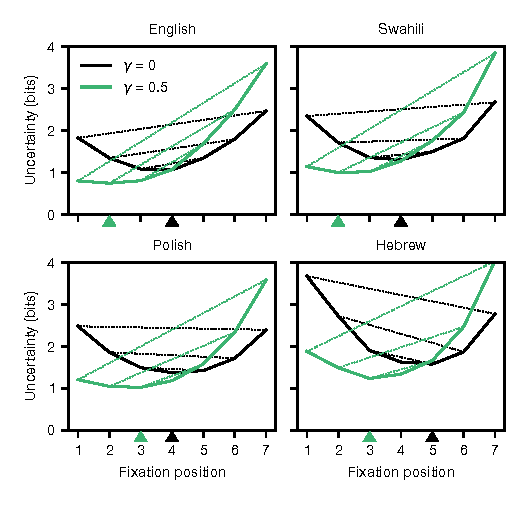
\includegraphics[]{figs/fig02.eps}}
\vspace*{2pt}
\caption{Uncertainty by fixation position for the seven-letter words in English, Swahili, Polish, and Hebrew. The triangles on the \textit{x}-axis mark the position of minimum uncertainty. Under a symmetric visual span (black; $\gamma=0$), uncertainty is generally minimized in central position. Under a right-visual-field advantage (green; $\gamma=0.5$), the position of minimum uncertainty is shifted further left. \newmaterial{N.B., in all cases, including Hebrew, the \textit{x}-axis represents the physical left-to-right character position.}}
\label{fig02}
\end{figure}

The results presented in Table~\ref{english_word_inferences} are for just two words. We now scale~up and consider the lexicon as a whole. Fig.~\ref{fig02} shows uncertainty by fixation position for the seven-letter words in four of the languages, English, Swahili, Polish, and Hebrew (see Fig.~S1 in the Supplementary Material for all languages and word lengths). The uncertainty curves presented in black ($\gamma = 0$; no perceptual bias) take on a characteristic \textsc{u}-shape because, in general, fixating the center yields a better overall view than fixating the edges. Further, we find that these \textsc{u}-shapes may be asymmetric---and more~so in some languages than others. In English, the uncertainty curve is left-heavy because left-heavy words are more prevalent than right-heavy ones. Swahili has a flatter distribution of information, Polish is slightly right-heavy, and Hebrew is very right-heavy.\footnote{Note that, in Hebrew, the right corresponds to the start of the words. In addition, vowel letters are typically omitted in writing, resulting in higher overall levels of uncertainty.} When the model reader is instantiated with a right-visual-field advantage ($\gamma = 0.5$; green curves), it becomes more advantageous to fixate further left, even in the case of Hebrew where the right-heavy distribution of information is overwhelmed.\footnote{That being said, an account of the visual span based purely on reading habits might posit a left-visual-field advantage in the case of Hebrew, so for reference we also show results for $\gamma = -0.5$ in the Supplementary Material.} Of course, our setting of $\gamma$ to 0.5 is merely illustrative at this point, but we will estimate its value from experimental data in the next section.

These results suggest two things. Firstly, there is at~least some cross-linguistic variation in information distribution \parencite[see also][]{Shafir:2022}, which would therefore predict cross-linguistic variation in word targeting behavior. Secondly, any effect of information structure can easily be overshadowed by a sufficiently strong asymmetry in the visual span. As such, we set out to test the prediction that information distribution changes reading behavior by constructing two artificial lexicons---two ideal test cases---in which we can carefully control how information is distributed, while holding all other factors constant.

\section{Experiment 1}

The primary goal of our first experiment was to establish whether it is possible to experimentally manipulate the optimal viewing position effect with artificial lexicons. In addition, we wanted to estimate appropriate values for the perceptual parameters of the cognitive model, allowing us to make more concrete predictions about where participants ought to fixate if they seek to minimize uncertainty (predictions that we test in Experiment~2).

\subsection{Method}

Experiment~1 was not preregistered, since our goals were proof of concept, prediction generation, and parameter estimation.

\subsubsection{Participants}

Sixty participants were recruited via the Prolific platform and were paid £3.00 for participation (equivalent to a rate of £7.50 per hour based on the median completion time of 24~minutes). In addition to this base rate, participants could receive up to £1.20 in additional bonuses as detailed below (median bonus: £0.99). The most common first languages were: Portuguese (30\%), English (15\%), Polish (8.3\%), Spanish (6.7\%), and Greek (5\%). Only two participants reported knowledge of a language that is written in a right-to-left script. The experiment was approved by the SISSA Ethics Committee (protocol number:~10027; date: 26/04/2021) and was conducted in accordance with all relevant ethical regulations. All participants provided informed consent.

\subsubsection{Stimuli}

\begin{table}
\begin{center}
\begin{threeparttable}
\caption{Artificial lexicon structures with examples of possible surface forms (Experiments 1 and 2)}
\footnotesize
\label{table1}
\begin{tabular}{ccccccccccccccccccc}
\toprule
\multicolumn{9}{c}{Left-heavy lexicon} & & \multicolumn{9}{c}{Right-heavy lexicon} \\
\multicolumn{7}{c}{Underlying structure} & & Example & & \multicolumn{7}{c}{Underlying structure} & & Example \\
\texttt{S} & $c_1$ & $v_1$ & $c_5$ & $v_5$ & $c_9$ & \texttt{S} & & \texttt{SNYBEVS} & & \texttt{S} & $c_9$ & $v_5$ & $c_5$ & $v_1$ & $c_1$ & \texttt{S} & & \texttt{SVEBYNS} \\
\texttt{S} & $c_2$ & $v_2$ & $c_5$ & $v_5$ & $c_9$ & \texttt{S} & & \texttt{STOBEVS} & & \texttt{S} & $c_9$ & $v_5$ & $c_5$ & $v_2$ & $c_2$ & \texttt{S} & & \texttt{SVEBOTS} \\
\texttt{S} & $c_3$ & $v_3$ & $c_6$ & $v_5$ & $c_9$ & \texttt{S} & & \texttt{SGUPEVS} & & \texttt{S} & $c_9$ & $v_5$ & $c_6$ & $v_3$ & $c_3$ & \texttt{S} & & \texttt{SVEPUGS} \\
\texttt{S} & $c_4$ & $v_4$ & $c_6$ & $v_5$ & $c_9$ & \texttt{S} & & \texttt{SKAPEVS} & & \texttt{S} & $c_9$ & $v_5$ & $c_6$ & $v_4$ & $c_4$ & \texttt{S} & & \texttt{SVEPAKS} \\
\texttt{S} & $c_3$ & $v_1$ & $c_7$ & $v_6$ & $c_9$ & \texttt{S} & & \texttt{SGYDIVS} & & \texttt{S} & $c_9$ & $v_6$ & $c_7$ & $v_1$ & $c_3$ & \texttt{S} & & \texttt{SVIDYGS} \\
\texttt{S} & $c_1$ & $v_2$ & $c_7$ & $v_6$ & $c_9$ & \texttt{S} & & \texttt{SNODIVS} & & \texttt{S} & $c_9$ & $v_6$ & $c_7$ & $v_2$ & $c_1$ & \texttt{S} & & \texttt{SVIDONS} \\
\texttt{S} & $c_4$ & $v_3$ & $c_8$ & $v_6$ & $c_9$ & \texttt{S} & & \texttt{SKUMIVS} & & \texttt{S} & $c_9$ & $v_6$ & $c_8$ & $v_3$ & $c_4$ & \texttt{S} & & \texttt{SVIMUKS} \\
\texttt{S} & $c_2$ & $v_4$ & $c_8$ & $v_6$ & $c_9$ & \texttt{S} & & \texttt{STAMIVS} & & \texttt{S} & $c_9$ & $v_6$ & $c_8$ & $v_4$ & $c_2$ & \texttt{S} & & \texttt{SVIMATS} \\
\bottomrule
\end{tabular} 
\end{threeparttable}
\end{center} 
\end{table}

We designed a pair of artificial lexicons---one left-heavy and one right-heavy---that would yield distinct, testable predictions in terms of where uncertainty will be minimized. Each lexicon consists of eight seven-letter words, the underlying structure of which is shown in Table~\ref{table1}. Each word followed a CCVCVCC pattern (e.g., \texttt{SVIMUKS}) that always began and ended with the letter \texttt{S}. \newmaterial{These outer \texttt{S}'s can be thought of as lateral flankers that carry no information, eliminating potential issues relating to the special status of initial and final letters \parencite{Johnson:2012, White:2008} or perceptual crowding effects \parencite{Pelli:2008}.} The five internal letters were constructed from a set of nine consonant letters, \{\texttt{B}, \texttt{D}, \texttt{G}, \texttt{K}, \texttt{M}, \texttt{N}, \texttt{P}, \texttt{T}, \texttt{V}\}, and a set of six vowel letters, \{\texttt{A}, \texttt{E}, \texttt{I}, \texttt{O}, \texttt{U}, \texttt{Y}\}. These two sets were permuted for each participant, such that the surface forms (examples of which are shown in Table~\ref{table1}) were different for each participant, although they always had the same underlying information structure. The characters that may occupy each position were chosen so that information is distributed asymmetrically. For example, across the eight words in the left-heavy lexicon, each of the letters in position~2 occurs twice; thus, this letter position conveys $-\log \frac{2}{8} = 2$~bits of information about word identity. In position~6, by comparison, the letter $c_9$ occurs in all eight words, so this letter position conveys $-\log \frac{8}{8} = 0$~bits of information. Importantly, the two lexicons are simply mirror-images of each other, and are thus identical except for the lateral distribution of information.

In order to present the stimuli at a consistent size across devices, participants were asked to place a credit card on the screen and adjust an on-screen image so that it matched the size of the physical card \parencite{Li:2020}. The words were presented in upper-case Courier New with a physical width of approximately 10~mm per letter. Participants were asked to sit approximately 50~cm from the display, resulting in each letter occupying approximately 1.15~degrees of visual angle. The corresponding object stimuli were taken from the Novel Object and Unusual Name database \parencite{Horst:2016} and were presented in grayscale at a size of approximately $40 \times 40$~mm.

\subsubsection{Procedure}

\begin{figure}
\makebox[\textwidth][c]{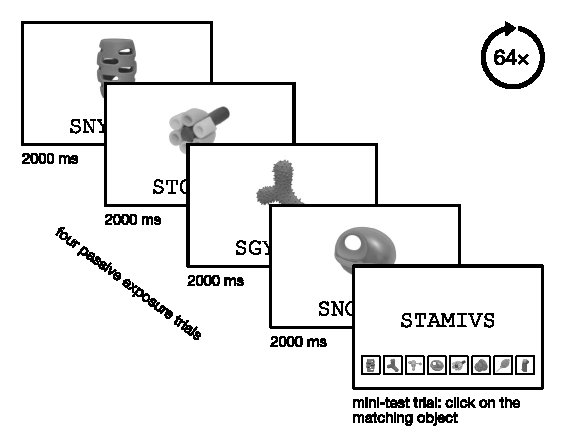
\includegraphics[]{figs/fig03.eps}}
\vspace*{2pt}
\caption{Training regimen (all experiments). Participants complete a mixture of passive exposure trials and mini-test trials in which they have to select the appropriate object for a word.}
\label{fig03}
\end{figure}

Participants were told that they would be learning an ``alien'' language and that their goal was to learn the words for a set of eight alien objects. In the training phase, participants were taught one of the two lexicons (Fig.~\ref{fig03}). During training, the participant was passively exposed to four word--object pairs in quick succession. Each passive exposure trial lasted 2000~ms with the word appearing after a 500~ms delay so that the participant's gaze was first drawn to the object and then to the word (i.e., the word itself was shown for 1500~ms). The participant was then shown one of the eight words (not necessarily from the previous four passive exposure trials) and had to click on the appropriate object, which we refer to as a ``mini-test.'' The purpose of these mini-test trials was to keep participants actively engaged in the learning process and to allow us to track learning performance over the course of the training period. Regardless of whether or not the participant chose the correct answer, the picture for the correct object remained on screen for one second, while the remaining object pictures disappeared, providing feedback and reinforcing the correct mapping. The participant was awarded a bonus of £0.01 for a correct answer. This procedure was repeated 64 times, such that each of the word--object pairs was passively exposed 32 times (256 passive exposure trials in total) and tested eight times (64 mini-test trials in total).

\begin{figure}
\makebox[\textwidth][c]{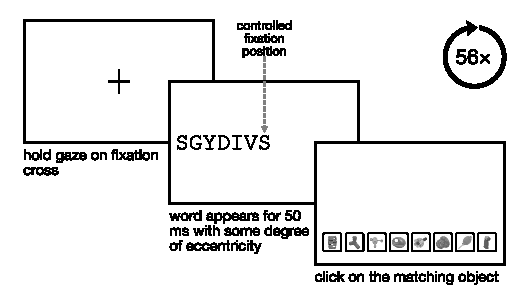
\includegraphics[]{figs/fig04.eps}}
\vspace*{2pt}
\caption{Controlled fixation test trial (Experiment 1). The participant fixates a fixation point and, after a short delay, a word is displayed for 50~ms. The word is positioned such that one of the seven characters is aligned with the fixation point. In this example, the word \texttt{SGYDIVS} is fixated in the final, uninformative position, making it hard to identify.}
\label{fig04}
\end{figure}

Participants were then tested on their ability to identify the words in each of the seven character positions (Fig.~\ref{fig04}). In each test trial, the participant was first asked to look at a fixation point positioned horizontally center. After a randomly determined delay of between 1000~and 3000~ms, one of the eight words was displayed on screen for 50~ms and the participant was asked to select the corresponding object for that word, just as in the previous mini-test trials. Since 50~ms is below the time required to plan and execute a saccade \parencite{Rayner:1998}, this forces participants to identify the words based on a single fixation in an experimenter-controlled position. Feedback and bonusing was also provided as before. Crucially, the word was presented with some degree of eccentricity: One of the seven letters was aligned with the position of the fixation point, such that the word itself may appear shifted to the left or right. Each of the seven characters from each of the eight words was tested once in fixation position, resulting in 56 test trials.

\subsection{Results}

The majority of participants (51/60) made zero or one error during the final block of training, indicating good learning of the object--word pairs. The remaining nine participants, who made two or more errors, were excluded from further analysis. Our rationale with this exclusion criterion was that we can only meaningfully measure a participant's ability to identify words in the test phase if they acquired the object--word pairs to a high degree of proficiency in the training phase (i.e., because correct object selection is only an index of correct word recognition). After these exclusions, the dataset that entered into our analysis included 1232 trials across 22 participants in the left-heavy condition and 1624 trials across 29 participants in the right-heavy condition.

\begin{figure}
\makebox[\textwidth][c]{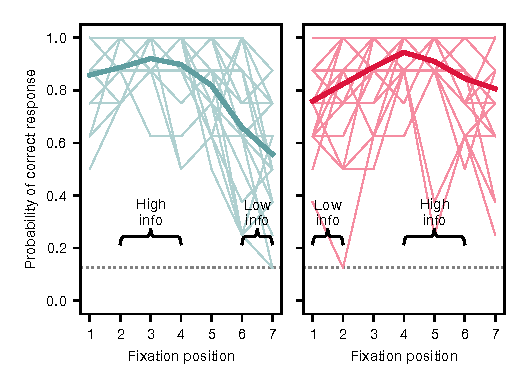
\includegraphics[]{figs/fig05.eps}}
\vspace*{2pt}
\caption{Mean accuracy by fixation position for each condition in Experiment~1. The thin, light-colored lines show results for individual participants. In the left-heavy condition (blue), participants are most accurate when fixating left-of-center where the words are more informative. In the right-heavy condition (red), participants are most accurate in central position, despite the fact that the words are more informative right-of-center.}
\label{fig05}
\end{figure}

Overall test accuracy was slightly lower in the left-heavy condition (mean: 0.8, 95\% HDI: 0.75--0.84) compared to the right-heavy condition (mean: 0.85, 95\% HDI: 0.81--0.89), which is to be expected under a right-visual-field advantage.\footnote{Recall from our model simulations that, under a right-visual-field advantage, identification is easier on right-heavy words.} Fig.~\ref{fig05} breaks down test accuracy by fixation position. In the case of the left-heavy condition, accuracy was highest in position~3 and lowest in position~7. The overall shape of this accuracy curve may be explained by perception, information, or both. The left-of-center area offers a good viewing position of the word as a whole (i.e., assuming a right-visual-field advantage), but the left-of-center area is also information rich. Likewise, the final position, where accuracy was lowest, offers a poor view of the word and contains low information content. In the case of the right-heavy condition, where we might naively expect to see mirrored results, we found that accuracy was actually maximized in central position and remained comparatively high even in position~1, where the information content is lowest. This may be explained by an interaction between perception and information: Accuracy is high in central position because this offers a good overall view of the word, including the informative content to the right; accuracy remains high in initial position because, assuming a right-visual-field advantage, the informative content near the end of the word can still be accurately captured.

In other words, in the left-heavy condition perception and information are aligned and reinforce each other, making a left-of-center fixation most beneficial. In the right-heavy condition, by contrast, the two factors cancel out: The structure of the lexicon makes it easier to identify words right-of-center, but the right-visual-field advantage makes a left-of-center fixation more advantageous. The net effect is that central fixation is most beneficial. To provide a quantitative confirmation of this explanation, we now fit the parameters of our cognitive model to the experimental data.

To perform the model fit, we introduced a noise parameter, $\epsilon \in (0, 1)$, in addition to the three perceptual parameters described earlier ($\alpha$, $\beta$, and $\gamma$). This parameter represents the probability of participants making selection errors (e.g., mapping the inferred word to the wrong meaning or accidentally clicking the wrong button) and helps to improve our estimates of the perceptual parameters by accounting for other sources of noise separately. Given the assumptions of the model $\mathcal{M}$ and some setting of the four model parameters, collectively denoted $\theta$, the likelihood of observing experimental dataset $D$ is given by
\begin{equation}
\mathrm{Pr}(D|\mathcal{M},\theta) = \prod_{\langle t,j,w \rangle} \sum_{w^\prime \in W}
    \begin{cases}
    \mathrm{Pr}(w^\prime|t,j)(1 - \epsilon)       & \text{if $w^\prime = w$} \\
    \mathrm{Pr}(w^\prime|t,j)\frac{\epsilon}{n-1} & \text{otherwise,}
    \end{cases}
\label{dataset_likelihood}
\end{equation}
where $\langle t,j,w \rangle$ represents each trial in $D$ (the target word, the position in which that word was fixated, and the participant's inference as indicated by the object they clicked on). The term $\mathrm{Pr}(w^\prime|t,j)$ specifies the probability that the model reader would infer $w^\prime$ when given the same input as the participant (the target word $t$ fixated in position $j$).\footnote{Formally this is given by $\sum_{p \in P} \mathrm{Pr}(p|t,j) \mathrm{Pr}(w^\prime|p,j)$. However, in practice we estimate its value by simulating 10,000 reading events.} Therefore, the summation in Equation~\ref{dataset_likelihood} accounts for all ways in which the model reader could make the same inference as the participant on a given trial -- either by inferring the same word as the participant and sticking to that choice with probability $1-\epsilon$ or by inferring some other word and accidentally switching to the same choice as the participant with probability $\epsilon / (n-1)$.

\begin{figure}
\makebox[\textwidth][c]{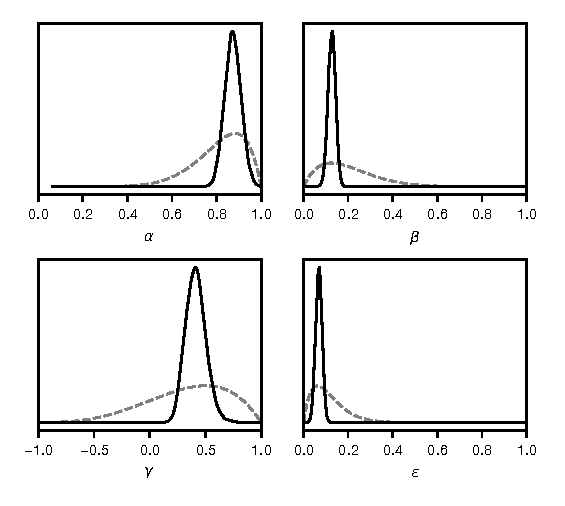
\includegraphics[]{figs/fig06.eps}}
\vspace*{2pt}
\caption{Prior (dashed) and posterior (solid) densities for each model parameter. The positive estimate of $\gamma$ confirms that participants have a right-visual-field advantage and quantifies its strength.}
\label{fig06}
\end{figure}

To place a prior on each parameter, we chose a beta distribution (transformed to the relevant parameter bounds) that was representative of the information available to us before running the experiment. The priors are illustrated by the dashed grey lines in Fig.~\ref{fig06} and were motivated as follows:
\begin{itemize}
    \item $\alpha \sim \mathrm{Beta}(8, 2)$: We expected readers to have a fairly high probability of correctly identifying the character under fixation, probably well beyond 60\%.
    \item $\beta \sim \mathrm{Beta}(2, 8)$: We expected this parameter to be on the low end of the scale, corresponding to visual span that is several letters wide. Small values ($< 0.01$) and large values ($> 0.5$) are implausible because these would correspond to overly wide and overly narrow visual spans respectively.
    \item $\gamma \sim \mathrm{Beta}(4, 2)$: Following the prior literature, we expected readers to be better at identifying characters to the right of fixation, resulting in a positive $\gamma$ value. However, since it was unclear how strongly this model parameter should be set, we opted for a broad prior that peaks at 0.5. We also wanted to remain relatively open-minded to the possibility of a symmetric visual span (i.e., $\gamma = 0$); perhaps, for example, the artificial language learning paradigm would be insufficient to reveal a visual span asymmetry.
    \item $\epsilon \sim \mathrm{Beta}(2, 16)$: We expected selection errors to be fairly rare (e.g., less than 20\%), especially since we had already excluded participants who demonstrated poor learning during the training phase.
\end{itemize}

The joint posterior distribution over the parameter space, $\mathrm{Pr}(\theta|\mathcal{M},D)$, was estimated using the Python package PyMC with six chains of 2500 samples (sequential sampling, all ESS $> 1000$, all $\hat{R}=1$) and is plotted in Fig.~\ref{fig06}. Crucially, $\gamma$ was estimated to have a \textit{positive} value of 0.41 (95\% HDI: 0.25--0.59). Not only does this mean that our experimental dataset is best explained by assuming a right-visual-field advantage, as expected from the prior literature, but it also quantifies the strength of this advantage in the context of our experimental setup and modeling framework. Complete posterior parameter estimates are given in Table~S1 in the Supplementary Material.

We also performed the model fit with uniform priors and obtained almost identical results. As an additional sanity check, we estimated the posterior using the data from each experimental condition independently, that is $\mathrm{Pr}(\theta|\mathcal{M},D_\mathrm{left})$ and $\mathrm{Pr}(\theta|\mathcal{M},D_\mathrm{right})$. These posteriors showed a high degree of overlap, suggesting that they reflect a single underlying perceptual filter that is common to all participants regardless of the lexicon they were exposed to in training (see Fig.~S2 in the Supplementary Material).

\begin{figure}
\makebox[\textwidth][c]{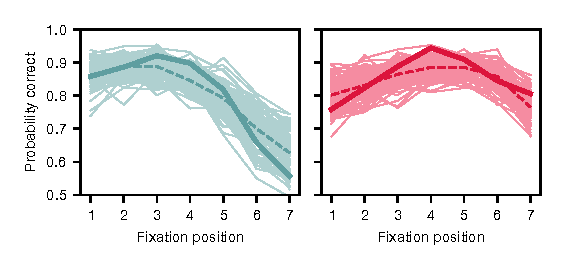
\includegraphics[]{figs/fig07.eps}}
\vspace*{2pt}
\caption{Posterior predictive checks of the model fit. Each thin line depicts the mean accuracy curve from a simulated run of the experiment using parameter values drawn from the posterior. The dashed line shows the mean of 100 simulated runs; the thick line shows the actual experimental findings.}
\label{fig07}
\end{figure}

Forward simulations of the experiment using parameter values drawn from the posterior can be seen in Fig.~\ref{fig07}. These simulations are able to retrodict overall accuracy levels fairly well and capture the distinctive shapes of the two conditions. Importantly, the experimental results fall neatly within the posterior predictive distribution, meaning that the pattern of results we observed is exactly what one would expect to see when the right-visual-field advantage interacts with the information distributions of the two constructed lexicons.

\begin{figure}
\makebox[\textwidth][c]{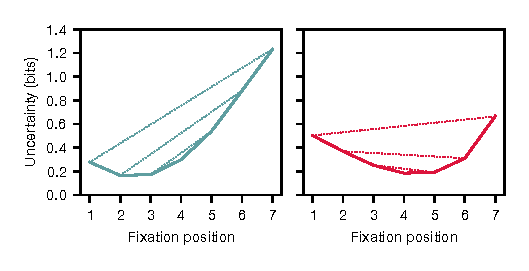
\includegraphics[]{figs/fig08.eps}}
\vspace*{2pt}
\caption{Reader uncertainty by fixation position. These curves predict where uncertainty will be minimized after accounting for both the structure of the artificial lexicons and the best fitting parameters of the perceptual filter.}
\label{fig08}
\end{figure}

Finally, Fig.~\ref{fig08} shows predicted uncertainty by fixation position for the left- and right-heavy lexicons, incorporating the perceptual asymmetry estimated from the Experiment~1 data. The shapes of these uncertainty curves are distinctive in two important ways, yielding testable predictions. Firstly, participants exposed to the left-heavy lexicon should prefer to fixate around positions~2 or~3, since this is where uncertainty is minimized, while participants exposed to the right-heavy lexicon should prefer to fixate more centrally in positions~4 or~5. Secondly, and less obviously, the uncertainty curve for the right-heavy lexicon is comparatively flat, which may result in lower pressure to land exactly on the position of minimum uncertainty (i.e., because uncertainty is relatively low regardless of fixation position). This may lead to more dispersed landing positions in the right-heavy condition.

\section{Experiment 2}

Our first experiment showed that the classic optimal viewing position effect \parencite[e.g.,][]{Brysbaert:1996} can be replicated with artificial languages: Accuracy in word recognition is a function of how much information is accessible at a given position and the shape of the visual span. But are readers able to learn which position minimizes uncertainty across the lexicon as a whole, and do they actively target this position? To answer these questions, we conducted a second experiment with the same stimuli and training procedure but a new type of test phase in which participants could, like Experiment~1, view the words for at~most 50~ms but, unlike Experiment~1, freely target them in any position. Based on the predictions derived from our first experiment, we made two hypotheses:
\begin{enumerate}
    \item Participants exposed to the right-heavy lexicon will target the words further right.
    \item Participants exposed to the right-heavy lexicon will have more dispersed landing positions.
\end{enumerate}

\subsection{Method}

The experiment was preregistered at \url{https://aspredicted.org/BS2_6N2}; we made no deviations from the preregistered analysis plan.

\subsubsection{Participants}

Eighty participants were recruited via our local participant pool and were paid €10 for participation (equivalent to a rate of €12 per hour based on the median completion time of 50~minutes). Participants were predominantly native speakers of Italian. The experiment was approved by the SISSA Ethics Committee (protocol number:~28135; date: 24/12/2021) and was conducted in accordance with all relevant ethical regulations. All participants provided informed consent.

\subsubsection{Procedure}

\begin{figure}
\makebox[\textwidth][c]{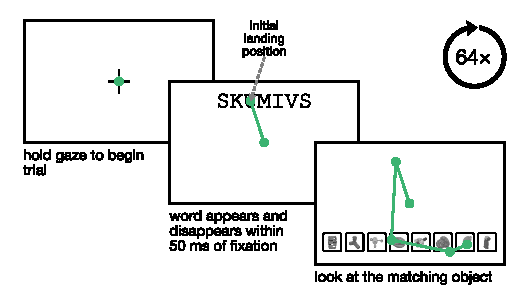
\includegraphics[]{figs/fig09.eps}}
\vspace*{2pt}
\caption{Free fixation test trial (Experiments~2 and~3). The participant fixates a fixation point until a word flashes up in a random (but horizontally centered) position above or below the fixation point. The word disappears within 50~ms of being fixated, such that the participant must identify the word using a single fixation. The participant's gaze path is shown in green. In this example, the participant targets the word \texttt{SKUMIVS} in third position.}
\label{fig09}
\end{figure}

The stimuli and training phase were identical to Experiment~1, but participants completed a different type of test phase, as illustrated in Fig.~\ref{fig09}. To initiate a trial, the participant had to hold their gaze for 2000~ms within an 18~px radius of a fixation point at the center of the screen. A target word then appeared either above or below the fixation point in a vertically random (but horizontally centered) position, and the word disappeared within 50~ms of its bounding box first being entered. The participant's task was to locate and identify the word, and then select the corresponding alien object from the full array of objects, just as in Experiment~1. Feedback was provided as before. Each participant completed 64 test trials (eight trials for each of the eight words).

During the test phase, participants' eye movements were recorded using an EyeLink~1000~Plus eye tracker (SR~Research, Toronto, Canada) with monocular (dominant eye) recording at a 1000~Hz sampling rate. Participants used a headrest positioned 57~cm from the screen, and the words were presented at a width of 36~px per character (approximately 11~mm or 1.1 degrees of visual angle). To maintain a high level of precision and provide participants with frequent opportunities to relax and adjust their head position, the eye tracker was recalibrated at least every eight trials (or more often as required) using 13-point calibration. The participant's initial landing position on a word was defined as the pixel distance between the first fixation recorded inside the word's bounding box and the left edge of that bounding box.

\subsubsection{Statistical model}

To evaluate the two hypotheses, we constructed the following multilevel Bayesian statistical model:
\begin{align*}
                  x_{i} & \sim \mathrm{Normal}(\mu_{j}, \sigma_{j}) \\
                \mu_{j} & \sim \mathrm{Normal}(\tau_k, \zeta) \\
             \sigma_{j} & \sim \mathrm{Gamma}(\delta_k, \xi) \\
     \tau_\mathrm{left} & \sim \mathrm{Normal}(72, 20) \\
    \tau_\mathrm{right} & \sim \mathrm{Normal}(144, 20) \\
                  \zeta & \sim \mathrm{Exponential}(0.1) \\
   \delta_\mathrm{left} & \sim \mathrm{Gamma}(20, 8) \\
  \delta_\mathrm{right} & \sim \mathrm{Gamma}(30, 8) \\
                    \xi & \sim \mathrm{Exponential}(0.1) \\
           \Delta(\tau) & = \tau_\mathrm{right} - \tau_\mathrm{left} \\
         \Delta(\delta) & = \delta_\mathrm{right} - \delta_\mathrm{left}
\end{align*}
where $i$ indexes trials by participant $j$, and $j$ indexes participants assigned to condition $k$. The model states that the pixel landing positions $x_i$ are normally distributed according to a mean $\mu_{j}$ and standard deviation $\sigma_{j}$ that is specific to each participant. These by-participant $\mu$'s and $\sigma$'s are also drawn from normal (or normal-like) distributions, representing across-participant variation in targeting behavior.\footnote{Note that we follow the convention of parameterizing the Gammas with a mean and standard deviation.} The average target pixel position is represented by the hyperparameter $\tau$ and the average dispersion is represented by the hyperparameter $\delta$, both stratified by condition, while $\zeta$ and $\xi$ place regularizing hyperpriors on the variation in across-participant behavior. The deterministic parameters $\Delta(\tau)$ and $\Delta(\delta)$ represent the difference in targeting and dispersion behavior between the two conditions. Formally, Hypothesis~1 states that $\Delta(\tau) > 0$ and Hypothesis~2 states that $\Delta(\delta) > 0$.

For the purpose of making discrete inferential decisions about the hypotheses, we followed the ROPE (region of practical equivalence) and HDI (highest density interval) approach \parencite{Kruschke:2015}. We set the ROPEs based on a minimally interesting effect size (one quarter of the width of a character). The ROPEs on $\Delta(\tau)$ and $\Delta(\delta)$ were $[-9, 9]$ and $[-4, 4]$ respectively. Our decision rules were as follows: If the 95\% HDI lies entirely above the ROPE, we accept the hypothesis; if it lies entirely within the ROPE, we reject the hypothesis; and if it overlaps the ROPE bounds, we consider the evidence indeterminate.

Our sample size was determined by a precision-based sequential sampling procedure, as recommended in \textcite{Kruschke:2015}. We planned to stop data collection once the widths of the 95\% HDIs on $\Delta(\tau)$ and $\Delta(\delta)$ shrank below 10~px and 5~px respectively, which we deemed to be a desirable level of precision. Due to resource limitations, however, we capped the number of participants at 80. This precision-based stopping criterion has no bearing on accepting or rejecting the hypotheses; it simply allows us to stop the experiment early if a high level of \textit{precision} is obtained, regardless of whether the inferential decision is positive, negative, or indeterminate.

\subsection{Results}

We did not meet the level of precision required to terminate the experiment early and therefore collected data from a total of 80 participants.\footnote{The 95\% HDI widths on $\Delta(\tau)$ and $\Delta(\delta)$ were 13.56~px and 4.51~px respectively, so we met the second criterion and were close to meeting the first. Note also that, although we did not reach the desired level of precision to stop data collection early, the posteriors are still fully interpretable.} Performance during the training phase was broadly the same as Experiment~1, and we applied the same training-based exclusion criterion resulting in seven participants being excluded. In the case of five participants, it was necessary to terminate the experimental session early due to calibration difficulties with the eye tracker (nevertheless, the trials that we did collect from these participants still enter into our analyses). Additionally, in a small number of trials (typically three of four trials per participant), no initial landing position could be identified because the participant's gaze swept over the word (causing it to disappear) without actually forming a fixation within the word boundary and within the word presentation time. The final dataset included 2119 trials across 37 participants in the left-heavy condition and 2165 trials across 36 participants in the right-heavy condition.

\begin{figure}
\makebox[\textwidth][c]{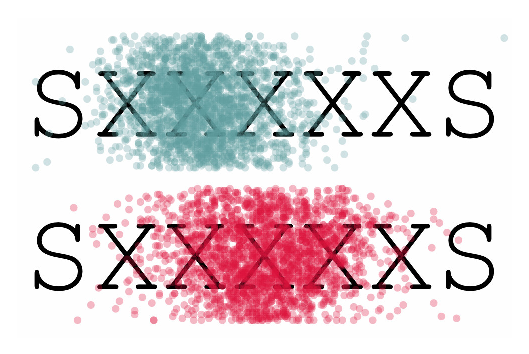
\includegraphics[]{figs/fig10.eps}}
\vspace*{2pt}
\caption{All initial landing positions for the left-heavy (blue) and right-heavy (red) conditions. All words began and ended with the letter~\textsc{s}, but the internal letters were different for each word/participant and are therefore represented here as~\textsc{x}'s.}
\label{fig10}
\end{figure}

\begin{figure}
\makebox[\textwidth][c]{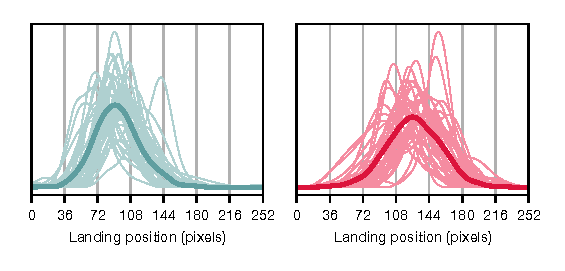
\includegraphics[]{figs/fig11.eps}}
\vspace*{2pt}
\caption{Kernel density plots of initial landing position. The thin, light-colored curves represent individual participants. Participants in the left-heavy condition (blue) tend to land left-of-center, while participants in the right-heavy condition (red) tend to land centrally.}
\label{fig11}
\end{figure}

Test accuracy was close to ceiling and almost identical between the left (mean: 0.97, 95\% HDI: 0.95--0.98) and right (mean: 0.98, 95\% HDI: 0.97--0.99) conditions. Higher accuracy levels were expected in Experiment~2 (compared to Experiment~1) because participants should now be targeting the words in their ideal locations, resulting in accurate word recognition on almost every trial. Fig.~\ref{fig10} and Fig.~\ref{fig11} plot the distribution of initial landing positions by condition and are immediately suggestive of a difference in reading behavior.

\begin{figure}
\makebox[\textwidth][c]{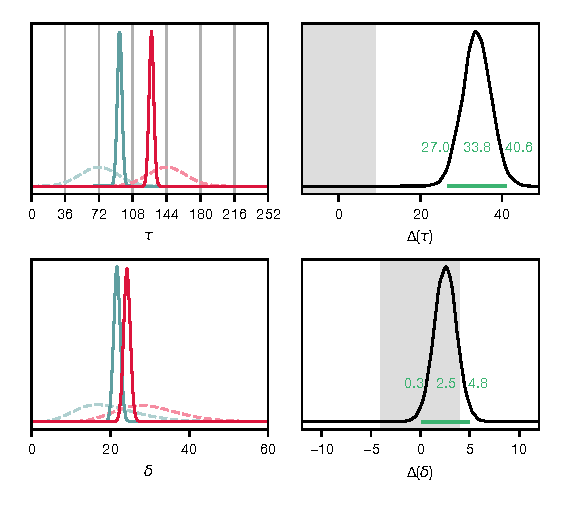
\includegraphics[]{figs/fig12.eps}}
\vspace*{2pt}
\caption{Prior (dashed) and posterior (solid) densities for $\tau$ and $\delta$, along with the posterior differences. The gray shaded area shows the ROPE and the green bar shows the 95\% HDI. Participants in the left-heavy condition (blue) target position~3 and participants in the right-heavy condition (red) target position~4. The posterior probability mass for $\Delta(\tau)$ lies well above 0, indicating a clear difference between conditions. Dispersion is slightly larger in the right-heavy condition; however, since the 95\% HDI overlaps the ROPE bounds, the evidence is considered indeterminate.}
\label{fig12}
\end{figure}

The statistical model was fit using the Python package PyMC with six chains of 2500 samples (NUTS, all ESS $> 10000$, all $\hat{R}=1$). The results are plotted in Fig.~\ref{fig12}. In terms of Hypothesis~1, there is a clear effect of condition with the posterior difference, $\Delta(\tau)$, estimated at 34~px (95\% HDI:~27--41) or approximately one character position. Participants exposed to the left-heavy lexicon tended to land 94~px into the word (95\% HDI:~89--99; character position~3), while participants exposed to the right-heavy lexicon tended to land 128~px into the word (95\% HDI:~123--133; character position~4). In terms of Hypothesis~2, the HDI overlaps the ROPE bounds so we consider the evidence to be indeterminate: On the one hand, 98.5\% of the posterior probability mass lies above 0, indicating that dispersion is greater in the right-heavy condition as hypothesized; but, on the other hand, 90.1\% of the posterior probability mass falls within the bounds of the ROPE, suggesting that, if there is an effect, it is likely to be of a negligible magnitude. Specifically, in the left-heavy condition, dispersion was 21.7~px (95\% HDI:~20.1--23.3), and in the right-heavy condition, dispersion was 24.2~px (95\% HDI:~22.6--25.9), yielding a posterior difference of 2.5~px (95\% HDI:~0.3--4.8). Complete posterior parameter estimates are given in Table~S2 in the Supplementary Material.

To check that the posteriors were not unduly influenced by our choice of priors, we also fit the model using uniform priors on $\tau$ and $\delta$ and obtained almost identical results (see Fig.~S3 in the Supplementary Material). We also found no meaningful difference in the results if the across-participant variation parameters ($\zeta$ and $\xi$) were stratified by condition (see Fig.~S4 in the Supplementary Material).

Overall, our results show that the information distribution of the learned language has a causal effect on how participants target words. Interestingly, participants do not simply target the part of the word that contains the most information; rather, they target the position that will minimize overall uncertainty, taking into account both the lexicon's information spread as well as the reader's own perceptual constraints, as predicted by our model. Note, for example, that participants exposed to the right-heavy lexicon primarily target the center of the word, presumably because this position still permits good access to the most information-heavy part of the word due to the right-visual-field advantage.

\section{Experiment 3}

One limitation of our artificial lexicons is that they consist purely of left-heavy or right-heavy words, whereas natural language lexicons include a mixture of both kinds of words. English, for example, has left-heavy words like \textit{guarded} and right-heavy words like \textit{concern}, although left-heavy words are more common leading to the overall bias in the English lexicon's information distribution. Our third experiment addresses this issue by adopting two new artificial lexicons in which the majority (but not all) of the words are left- or right-heavy. Like Experiment~2, we hypothesized that participants exposed to the right-dominant lexicon would target the words further right than those exposed to the left-dominant lexicon. We did not make a formal hypothesis about dispersion, since the results of Experiment~2 were suggestive of a weak or null effect on dispersion.

\subsection{Method}

Except for the new lexicons, the methods were identical to that of Experiment~2. The experiment was preregistered at \url{https://aspredicted.org/6RQ_GM7}; we made no deviations from the preregistered analysis plan.

\subsubsection{Participants}

Fifty-four participants were recruited via our local participant pool and were paid €10 for participation (equivalent to a rate of €12.50 per hour based on the median completion time of 48~minutes). Participants were predominantly native speakers of Italian. The experiment was approved by the SISSA Ethics Committee (protocol number:~28135; date: 24/12/2021) and was conducted in accordance with all relevant ethical regulations. All participants provided informed consent.

\subsubsection{Stimuli}

\begin{table}
\begin{center}
\begin{threeparttable}
\caption{Artificial lexicon structures with examples of possible surface forms (Experiment 3)}
\footnotesize
\label{table2}
\begin{tabular}{ccccccccccccccccccc}
\toprule
\multicolumn{9}{c}{Left-dominant lexicon} & & \multicolumn{9}{c}{Right-dominant lexicon} \\
\multicolumn{7}{c}{Underlying structure} & & Example & & \multicolumn{7}{c}{Underlying structure} & & Example \\
\texttt{S} & $c_1$ & $v_1$ & $c_8$ & $v_4$ & $c_9$ & \texttt{S} & & \texttt{SMOGIFS} & & \texttt{S} & $c_9$ & $v_4$ & $c_8$ & $v_1$ & $c_1$ & \texttt{S} & & \texttt{SFIGOMS} \\
\texttt{S} & $c_2$ & $v_2$ & $c_8$ & $v_4$ & $c_9$ & \texttt{S} & & \texttt{SDUGIFS} & & \texttt{S} & $c_9$ & $v_4$ & $c_8$ & $v_2$ & $c_2$ & \texttt{S} & & \texttt{SFIGUDS} \\
\texttt{S} & $c_3$ & $v_3$ & $c_8$ & $v_4$ & $c_9$ & \texttt{S} & & \texttt{SKAGIFS} & & \texttt{S} & $c_9$ & $v_4$ & $c_8$ & $v_3$ & $c_3$ & \texttt{S} & & \texttt{SFIGAKS} \\
\texttt{S} & $c_4$ & $v_1$ & $c_8$ & $v_4$ & $c_9$ & \texttt{S} & & \texttt{SNOGIFS} & & \texttt{S} & $c_9$ & $v_4$ & $c_8$ & $v_1$ & $c_4$ & \texttt{S} & & \texttt{SFIGONS} \\
\texttt{S} & $c_5$ & $v_2$ & $c_8$ & $v_4$ & $c_9$ & \texttt{S} & & \texttt{SLUGIFS} & & \texttt{S} & $c_9$ & $v_4$ & $c_8$ & $v_2$ & $c_5$ & \texttt{S} & & \texttt{SFIGULS} \\
\texttt{S} & $c_6$ & $v_3$ & $c_8$ & $v_4$ & $c_9$ & \texttt{S} & & \texttt{SPAGIFS} & & \texttt{S} & $c_9$ & $v_4$ & $c_8$ & $v_3$ & $c_6$ & \texttt{S} & & \texttt{SFIGAPS} \\
\texttt{S} & $c_7$ & $v_4$ & $c_8$ & $v_5$ & $c_{10}$ & \texttt{S} & & \texttt{STIGYBS} & & \texttt{S} & $c_{10}$ & $v_5$ & $c_8$ & $v_4$ & $c_7$ & \texttt{S} & & \texttt{SBYGITS} \\
\texttt{S} & $c_7$ & $v_4$ & $c_8$ & $v_6$ & $c_{11}$ & \texttt{S} & & \texttt{STIGEVS} & & \texttt{S} & $c_{11}$ & $v_6$ & $c_8$ & $v_4$ & $c_7$ & \texttt{S} & & \texttt{SVEGITS} \\
\bottomrule
\end{tabular} 
\end{threeparttable}
\end{center} 
\end{table}

Table~\ref{table2} shows the structure of the two new lexicons. In each case, the first six words (i.e., the majority of words, 75\%) use the dominant information distribution, while the final two words use the nondominant distribution. For example, in the left-dominant lexicon, the first six words can be thought of as containing a suffix (e.g., \texttt{-IFS}) and are therefore more informative on the left, while the final two words can be thought of as containing a prefix (e.g., \texttt{STI-}) and are therefore more informative on the right. Although the stimuli follow the same overall CCVCVCC pattern as before, it was necessary to introduce two additional consonant letters (\texttt{F} and \texttt{L}) and reduce the information contained in the central character, which is now fully uninformative.

\subsubsection{Statistical model}

Experiment~3 was analyzed using the following Bayesian statistical model:
\begin{align*}
               x_{i} & \sim \mathrm{Normal}(\mu_{j}, \sigma_{j}) \\
             \mu_{j} & \sim \mathrm{Normal}(\tau_k, \zeta) \\
          \sigma_{j} & \sim \mathrm{Gamma}(\delta, \xi) \\
  \tau_\mathrm{left} & \sim \mathrm{Normal}(94, 30) \\
 \tau_\mathrm{right} & \sim \mathrm{Normal}(128, 30) \\
              \delta & \sim \mathrm{Gamma}(23, 10) \\
               \zeta & \sim \mathrm{Exponential}(0.1) \\
                 \xi & \sim \mathrm{Exponential}(0.1) \\
        \Delta(\tau) & = \tau_\mathrm{right} - \tau_\mathrm{left}
\end{align*}
The model diverges from that of Experiment~2 in two main ways. First, we dropped the dispersion contrast---the estimate for the $\delta$ parameter is now pooled across both conditions. Second, our priors on $\tau$ and $\delta$ were updated to reflect what we had learned from Experiment~2; that is, we expected participants to target pixel~94 in the left-dominant condition and pixel~128 in the right-dominant condition, with around 23~pixels of dispersion. We also made a few other minor tweaks based our experience with Experiment~2. We increased the standard deviations on the $\tau$ and $\delta$ priors, since we felt our previous priors had been overly confident; we raised the precision criterion to 16~px, since we felt our previous criterion had been unnecessarily demanding; and we adjusted the ROPE bounds to $[-10, 10]$ to bring our specification into alignment with Kruschke's (\citeyear{Kruschke:2015}) recommendation that the precision criterion be 80\% of the ROPE width.

\subsection{Results}

Training performance was broadly the same as Experiments~1 and~2, and we applied the same training-based exclusion criterion resulting in three participants being excluded. As in Experiment~2, no initial landing position could be identified in a small number of cases (typically three or four trials per participant) because the participant did not form a fixation within the word boundary and within the word presentation time. The final dataset included 1497 trials across 25 participants in the left-heavy condition and 1583 trials across 26 participants in the right-heavy condition.

\begin{figure}
\makebox[\textwidth][c]{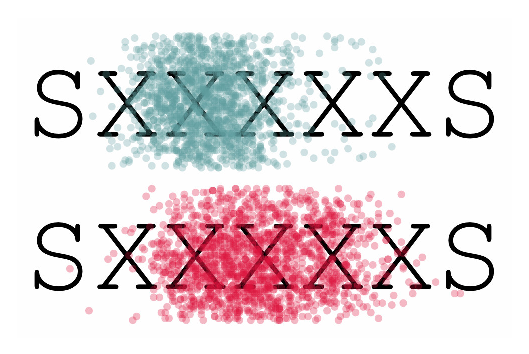
\includegraphics[]{figs/fig13.eps}}
\vspace*{2pt}
\caption{All initial landing positions for the left-heavy (blue) and right-heavy (red) conditions. All words began and ended with the letter~\textsc{s}, but the internal letters were different for each word/participant and are therefore represented here as~\textsc{x}'s.}
\label{fig13}
\end{figure}

\begin{figure}
\makebox[\textwidth][c]{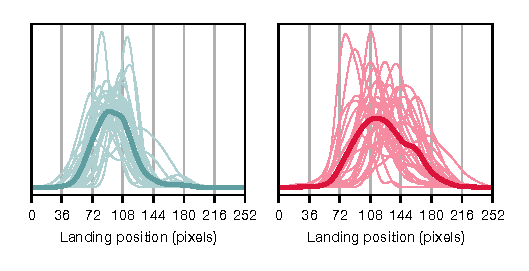
\includegraphics[]{figs/fig14.eps}}
\vspace*{2pt}
\caption{Kernel density plots of initial landing position. The thin, light-colored curves represent individual participants. Participants in the left-heavy condition (blue) tend to land left-of-center, while participants in the right-heavy condition (red) tend to land centrally.}
\label{fig14}
\end{figure}

Fig.~\ref{fig13} and Fig.~\ref{fig14} plot the distribution of initial landing positions by condition, and the statistical results are plotted in Fig.~\ref{fig15}. The results continue to show a clear effect of condition on targeting behavior with the posterior difference, $\Delta(\tau)$, estimated at 26~px (95\% HDI:~18--34). Participants exposed to the left-heavy lexicon tended to land 97~px into the word (95\% HDI:~92--103; character position~3), while participants exposed to the right-heavy lexicon tended to land 124~px into the word (95\% HDI:~118--129; character position~4). Complete posterior parameter estimates are given in Table~S3 in the Supplementary Material.

\begin{figure}
\makebox[\textwidth][c]{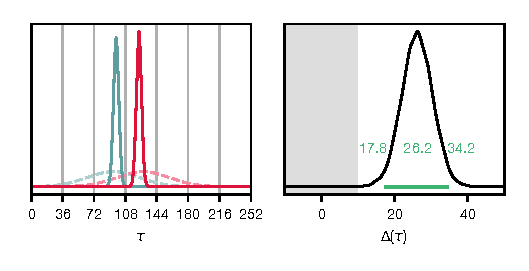
\includegraphics[]{figs/fig15.eps}}
\vspace*{2pt}
\caption{Prior (dashed) and posterior (solid) densities for $\tau$, along with the posterior difference $\Delta(\tau)$. The gray shaded area shows the ROPE and the green bar shows the 95\% HDI. Participants in the left-heavy condition (blue) target position~3 and participants in the right-heavy condition (red) target position~4. The posterior probability mass for $\Delta(\tau)$ lies well above 0, indicating a clear difference between conditions.}
\label{fig15}
\end{figure}

We also fit the model using uniform priors on $\tau$ and $\delta$ and obtained almost identical results (see Fig.~S5 in the Supplementary Material), and we found no meaningful change in the results after stratifying all parameters by condition (see Fig.~S6 in the Supplementary Material). Although we did not make a formal hypothesis about dispersion, we did note some evidence of a difference ($\Delta(\delta) = 4.6$~px; 95\% HDI: 1.3--7.8), although the effect was still not strong enough to meet the decision criteria we set~out in Experiment~2. Perhaps more interestingly, there was some evidence to suggest that across-participant variation in targeting ($\zeta$) was larger in the right-dominant condition ($\Delta(\zeta) = 6.8$~px; 95\% HDI: 0.6--13.1), although, again, the evidence for this is not entirely conclusive. Nevertheless, it does appear in Fig.~\ref{fig14} that participants in the right-dominant condition used a wider range of strategies than those in the left-dominant condition, with some participants targeting position~3, some targeting position~4, some targeting position~5, and some having a bimodal distribution targeting positions~3 and~5. It is not immediately clear why there might be a difference between conditions in this regard, but one possibility relates to carry-over from the participants' native language, Italian. If participants come into the study with an a-priori preference for targeting words left-of-center, it is perhaps more difficult for those assigned to the right-dominant condition to overcome this prior experience, especially since the minority-type words (i.e., the left-heavy words in the right-dominant lexicon) did indeed require a left-of-center fixation.

Overall, the results of Experiment~3 show that the effect of average information distribution on word targeting continues to hold even when the lexicon contains a mixture of both left- and right-heavy words. Participants exposed to the right-dominant lexicon, in which the majority of words are more informative on the right, fixated around 26~px further to the right than participants exposed to the left-dominant lexicon. This effect size was smaller than that observed in Experiment~2, but this may be explained by the fact that, under a mixed lexicon, participants need to hedge their bets, since they cannot know a~priori whether or not the target word will conform to the dominant information distribution.

\section{Discussion}

Mounting evidence shows that language processing takes full advantage of probabilistic cues present in the language itself. One such cue in the domain of reading is the way in which information about word identity is distributed across words, providing readers with expectations about which position tends to be most informative (i.e., minimizes uncertainty about word identity). Previous research has explored this issue by contrasting word processing in different languages, and while this has provided precious insight, the approach has struggled to disentangle information distribution from perceptual asymmetries and other important factors that distinguish human languages (e.g., morphology and reading direction). To circumvent this complexity, we adopted an artificial language learning approach, which allowed us to isolate the role of information distribution and test its \textit{causal} effect on eye movement behavior.

We first devised a cognitive model of visual word recognition that predicts uncertainty as a function of the human perceptual bias and the linguistic informational bias. Applying this model to a selection of languages, we found that there is at~least some cross-linguistic variation in how information is distributed within lexicons, which therefore predicts cross-linguistic variation in how readers ought to target words. We tested this prediction by submitting participants to one of two artificial lexicons, which differ only in how information is laterally distributed.

In Experiment~1, we focused on accuracy in word recognition. We demonstrated the feasibility of eliciting the classic optimal viewing position effect \parencite{ORegan:1984, Brysbaert:2005, Hyona:2011} using artificially constructed lexicons, and we showed that the effect could, in principle, be manipulated by changing the distribution of information. \newmaterial{The interaction we observed between the right-visual-field advantage and the location of information in the words is in close alignment with similar experiments by \textcite{Brysbaert:1996} using real languages (Dutch and French).} Experiment~1 also allowed us to estimate the parameters of the human visual span, as it pertains, at~least, to our experimental paradigm and modeling framework. This revealed clear evidence in support of the right-visual-field advantage and also allowed us to calibrate our model in order to make concrete predictions about reading behavior under the assumption that readers aim to minimize uncertainty when targeting words.

In Experiment~2, we estimated the causal effect on reading behavior of being exposed to the right-heavy lexicon instead of the left-heavy lexicon. The effect was to shift participants' initial landing positions around one character position to the right, which was broadly in~line with our model predictions. Evidence for an effect on dispersion was unclear, although we note that either the presence or absence of a dispersion effect could have interesting theoretical ramifications. A difference in dispersion would suggest that participants are sensitive to how concentrated information is in one particular area, while no difference in dispersion would suggest that participants adhere to a maximizing rule---always target the position of minimum uncertainty, even if it is only marginally better than some other position. Future work could aim to resolve this.

In Experiment~3, we addressed one potential issue with our artificial lexicons, namely that the lexicons consisted purely of one type of word (either left-heavy or right-heavy), whereas natural language lexicons contain a mixture of words with different distributions of information. The results of this experiment continued to show a clear difference in landing position, suggesting that participants are able to pick up on a cue that is more statistical in nature. In nonpreregistered analyses, we found some evidence to suggest that there is more variation in participants' targeting strategies in the right-dominant condition. This could be interpreted as a native-language carry-over effect. Participants in the left-dominant condition can simply stick to their normal patterns of behavior (target words left-of-center), while participants in the right-dominant condition must overcome their prior expectations. Individual differences in willingness to adapt to a new lexical environment might then explain the greater variation in targeting behavior. Future work could aim to investigate the issues of native-language carry-over and individual differences in this paradigm.

A broad distinction has been drawn in the literature between ``fast-heuristic'' accounts of targeting behavior, in which readers primarily target the center of an upcoming word, and ``cognitive-processing'' accounts, which incorporate ongoing processing of the upcoming word \parencite{Bicknell:2020}. Such ongoing processing may include, for example, predictions from prior sentence context \parencite{Balota:1985} or information garnered through parafoveal preview \parencite{Hyona:1989, Underwood:1990, Schotter:2011}. The present study represents a hybrid of these two accounts---a fast heuristic that is nevertheless rooted in experience with the language. Even in the absence of prior information about the identity of an upcoming word, readers can nevertheless target the position in which they expect to minimize uncertainty. This is not merely the position of maximum information content, nor the position that permits the best view of the word, but rather the position that optimizes the trade-off between the two.

Another interesting observation concerns the flexibility of the system. It is perhaps surprising that participants were able to overcome a lifetime of experience with just 15~minutes of exposure to these novel lexicons. However, related work has shown that the way participants attend to words can rapidly adapt to a new lexical environment \parencite{Ducrot:2002}. Moreover, substantial cognitive flexibility has been observed in many other domains. For example, participants can overcome the cultural representation of time as extending from left to right with just five minutes of mirror-reversed reading \parencite{Casasanto:2014}. These results point to human cognition as a flexible system that is able to respond quickly to a changing environment and account for volatile statistical cues.

\newmaterial{The extent to which our findings may generalize to normal reading scenarios (as opposed to isolated word reading) remains an open question. In particular, the use of lexicon-level statistical cues is likely to be supplemented by other sources of prior information, and these sources are likely to interact with each other in complex ways. The reader's prediction about the upcoming word based on prior sentence context might adjust how much weight they place on the more general language-level heuristic investigated here. If the upcoming word is very likely to be \textit{concern}, it perhaps pays to discard what you know about the language in general, and instead target the word right-of-center where you can expect to gather maximum information. Likewise, if highly constraining information has already been gathered from the parafovea about the initial letters in the upcoming word, it might, again, pay to flout what is known about the language in general.}

\newmaterial{With these issues in mind, it will be important to verify our findings in more naturalistic settings where the myriad determinants of eye movement behaviors interact. One way to approach this is using large, cross-linguistic eye movement corpora such as MECO \parencite{Siegelman:2022}; indeed, work in this direction is already underway \parencite{Shafir:2022}. Alternatively, experimental paradigms, such as the one used here, could be further extended and refined to incorporate other pertinent factors. Our alien words could be placed in predictive contexts, for example, and the availability of parafoveal information could be manipulated using the boundary paradigm. A particularly important issue will be to understand whether the oculomotor system is even precise enough to yield optimal landing positions based on the brain's prediction about where maximum information can be extracted. It has been shown for example, that a substantial proportion of saccades do not land on the targeted word, suggesting that the oculomotor system might introduce considerable noise in the targeting process \parencite{Engbert:2008}.}

The model we presented herein is conceptually similar to the Bayesian Reader \parencite{Norris:2006, Norris:2009, Norris:2012}. Like that work, our model is firmly expressed at the computational level of description \parencite{Marr:1982} and does not, therefore, make any strong commitments to particular neural processes or linguistic representations. Indeed, our model is even more simplified, dispensing with such features as positional uncertainty, reaction times, letter confusability, and crowding effects. The main feature our model adds---like other Bayesian models \parencite{SmithChan:2010, Bicknell:2012, Valdois:2021}---is that the probability of correctly identifying a letter is proportional to its distance from fixation. These choices were all motivated by keeping the model tightly focused around our particular domain of interest, that is, the relative contributions of perception and information to visual word recognition and the causal effect of information structure on word targeting. A nice feature of our model is that it does not make strong assumptions about linguistic representation and relies entirely on the system's sensitivity to statistics in the lexicon. \newmaterial{For example, the reader will be biased toward inferring \textit{ed}, \textit{er}, or \textit{es} at the end of a word---especially if it has a bad view of the end of the word---simply by virtue of the fact that these are common word endings in the lexicon, and not because of any built-in \textit{n}-gram chunking or awareness of morphology.}

The present work shows that sophisticated linguistic processes, like word recognition and targeting, may be explained in terms of simple, general-purpose cognitive heuristics such as maximal efficiency in the collection of information. This is in line with other work in the domain of visual processing, showing that the brain allocates more resources to aspects of the input that are more informative \parencite{Simoncelli:2001, Hermundstad:2014}. It also sits well with the observation that reading capitalizes on neural circuitry that was originally devoted, both ontogenetically and phylogenetically, to non-linguistic visual objects such as faces and tools \parencite{Dehaene:2011, Hervais:2019}. Although this might seem obvious (printed words are visual objects after all), it has widespread implications for the way we conceive of the lexical system. Much recent work has captured linguistic phenomena in terms of sensitivity to the statistics of the input. For example, word learning is affected by letter co-occurrence statistics \parencite{Chetail:2017, Lelonkiewicz:2020}, and aspects of orthographic processing that were long thought to be specific to letters and words emerge with entirely non-linguistic visual stimuli \parencite{Vidal:2021}.

Readers are also sensitive to the consistency in the mapping between spelling, sound, and meaning \parencite{Marelli:2015, Ulicheva:2020}, and signs of orthographic processing more generally have been observed in both naive \parencite{Rajalingham:2018} and trained \parencite{Grainger:2012} primates. Moreover, the efficient organization of lexical semantics has been shown to emerge in computational agents as they interact and develop a shared language \parencite{Chaabouni:2021}. This research suggests, at least in principle, that intelligent agents, gifted only with relatively simple---and certainly not language-specific---computational strategies, can develop behaviors and communication systems that share core features with human language.

This does not necessarily mean that the linguistic constructs we have used for decades (e.g., graphemes, morphemes, even words) are misplaced. The general-purpose computational machinery referenced above, combined with the input it receives, might certainly converge on representations and processes that are not dissimilar from classical linguistic constructs. It is also surely true that language and reading are so pervasive in human experience that some domain-specific phenomena may be expected to emerge. For example, position coding does seem to be different between letters and other visual objects \parencite{Dunabeitia:2012}. However, such domain specificity might come from intensive exposure rather than an intrinsic difference in how the brain processes language; from experience and efficient statistical machines, rather than specialized neural machinery.

\section{Acknowledgments}

This work was funded by an ERC (European Research Council) Starting Grant (no.\@ 679010, STATLEARN) and a FARE (Framework per l'Attrazione e il Rafforzamento delle Eccellenze per la Ricerca in Italia) 2016 grant (no.\@ R164XBHNYR, CROWDLEARN), both awarded to DC.

\printbibliography

%%%%%%%%%%%%%%%%%%%%%%%%%%%%%%%%%%%%%%%%%%%%%%%%%%%%%%%%%%%%%%%%%%%%%%%%%%%%%
% SUPPLEMENTARY MATERIAL
%%%%%%%%%%%%%%%%%%%%%%%%%%%%%%%%%%%%%%%%%%%%%%%%%%%%%%%%%%%%%%%%%%%%%%%%%%%%%

\appendix
\renewcommand\thefigure{S\arabic{figure}}
\setcounter{figure}{0}
\renewcommand\thetable{S\arabic{table}}
\setcounter{table}{0}


\begin{figure}
\makebox[\textwidth][c]{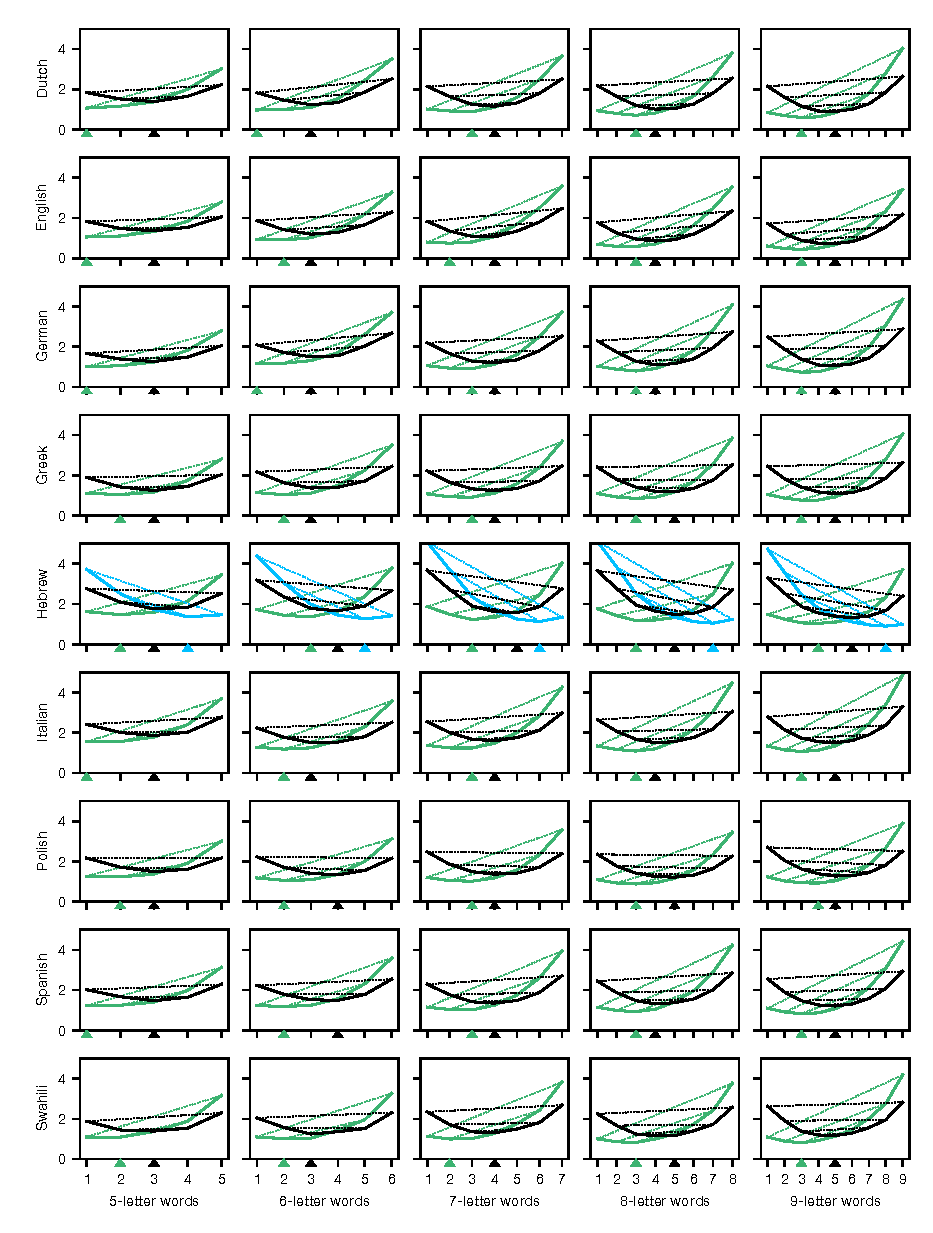
\includegraphics[]{figs/supp1.eps}}
\vspace*{2pt}
\caption{Uncertainty by fixation position in 5- to 9-letter words for nine languages. The triangles on the \textit{x}-axis mark the position of minimum uncertainty. Under a symmetric visual span (black; $\gamma=0$), uncertainty is generally minimized in central position or slightly left-of-centre. Under a right-visual-field advantage (green; $\gamma=0.5$), the position of minimum uncertainty is shifted further left. In the case of Hebrew, results are also shown for a left-visual-field advantage (blue; $\gamma=-0.5$).}
\label{supp1}
\end{figure}

\clearpage

\begin{figure}
\makebox[\textwidth][c]{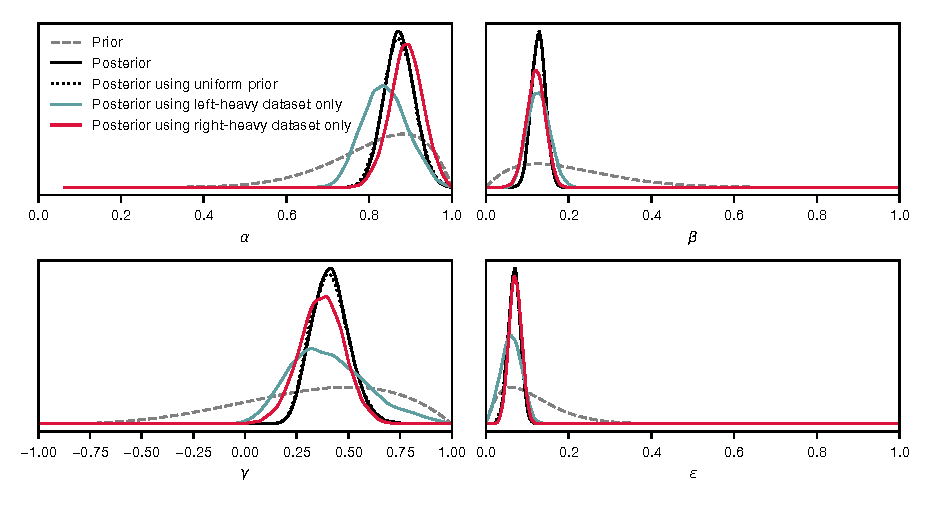
\includegraphics[]{figs/supp2.eps}}
\vspace*{2pt}
\caption{Canonical priors and posteriors for Experiment 1 alongside three other ways of estimating the posterior. The dotted curves show the posterior estimated with a uniform prior. These look almost identical to the canonical posterior (solid curves), so our choice of priors is not unduly biasing the posteriors. The colored curves show the posterior estimated from the left- and right-heavy datasets independently. These posterior estimates should theoretically be the same, since participants' perceptual filters should not differ depending on the lexicon they were exposed to. In general the two posteriors are closely aligned, although the posterior estimated from the left-heavy dataset (blue) does tend to deviate a little. That being said there's also quite a lot of uncertainty associated with the left-heavy estimates, probably because there were fewer participants in the left-heavy condition after exclusions.}
\label{supp2}
\end{figure}

\clearpage

\begin{figure}
\makebox[\textwidth][c]{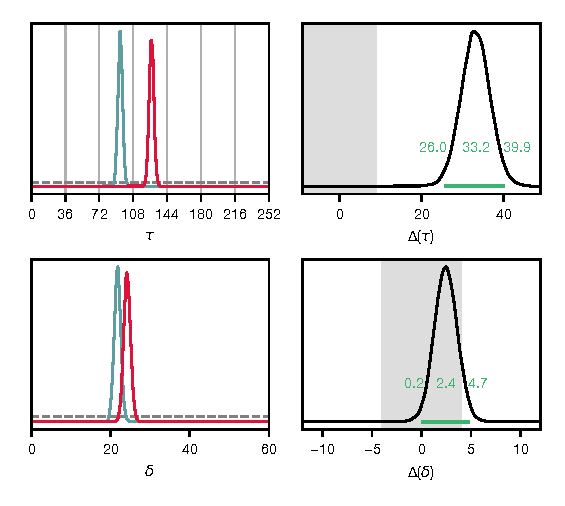
\includegraphics[]{figs/supp3.eps}}
\vspace*{2pt}
\caption{Posterior estimates for Experiment 2 using uniform priors. These results do not differ in any meaningful way from the canonical results reported in the main paper, so it is safe to conclude that our choice of priors is not biasing the results.}
\label{supp3}
\end{figure}

\clearpage

\begin{figure}
\makebox[\textwidth][c]{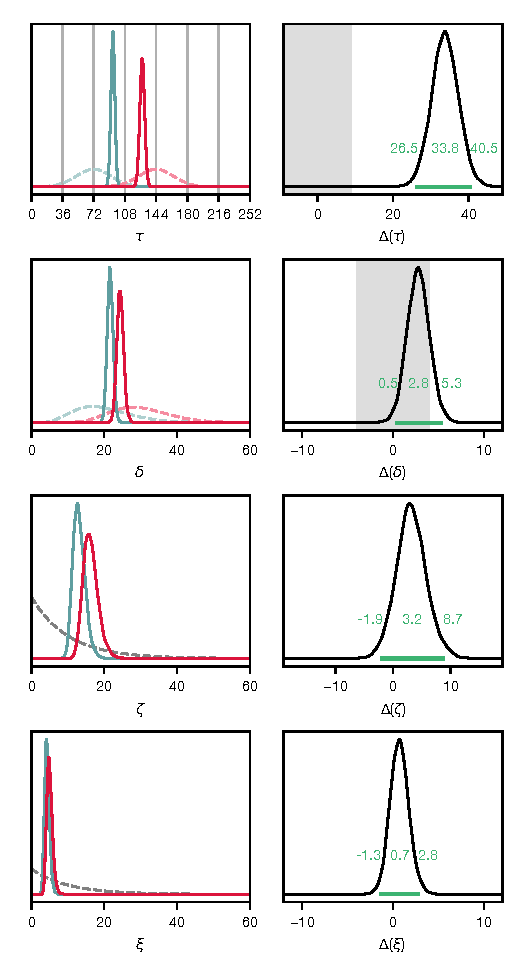
\includegraphics[]{figs/supp4.eps}}
\vspace*{2pt}
\caption{Posterior estimates for Experiment 2 allowing $\zeta$ and $\xi$ to vary independently by condition. The main results for $\tau$ and $\delta$ do not change in any meaningful way, and there is little evidence of a difference in the $\zeta$ and $\xi$ parameters, suggesting that the across-participant variation does not differ between conditions.}
\label{supp4}
\end{figure}

\clearpage

\begin{figure}
\makebox[\textwidth][c]{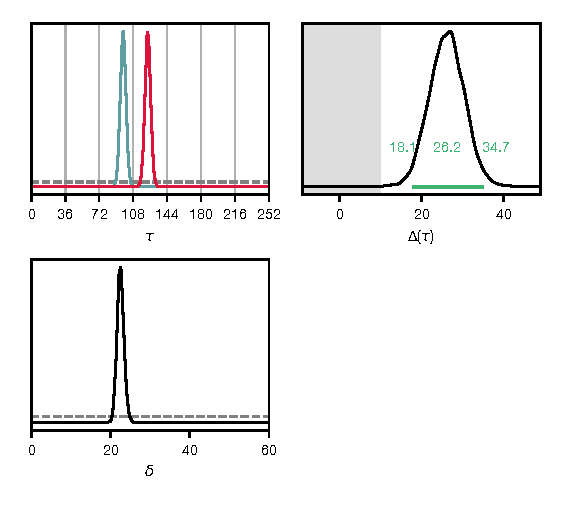
\includegraphics[]{figs/supp5.eps}}
\vspace*{2pt}
\caption{Posterior estimates for Experiment 3 using uniform priors on $\tau$ and $\delta$. These results are almost identical to our canonical results, suggesting that our choice of priors is not biasing the posteriors.}
\label{supp5}
\end{figure}

\clearpage

\begin{figure}
\makebox[\textwidth][c]{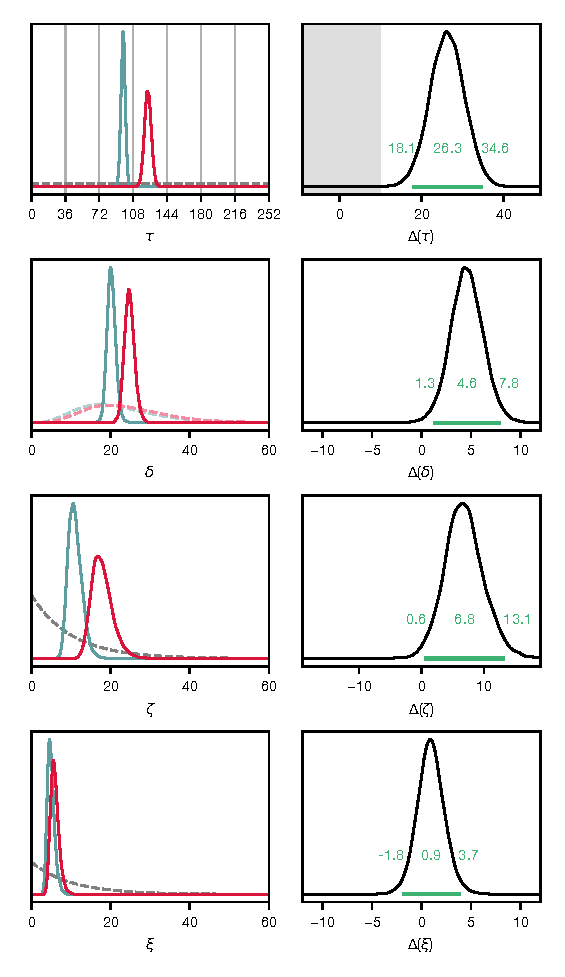
\includegraphics[]{figs/supp6.eps}}
\vspace*{2pt}
\caption{Posterior estimates for Experiment 3 allowing $\delta$, $\zeta$, and $\xi$ to vary independently by condition. The $\tau$ estimates are consistent under this model structure. Interestingly, we do find evidence for a difference in dispersion, albeit at a level that would have been considered indeterminate under our Experiment~2 $\delta$ ROPE. We also find some evidence of a difference in $\zeta$ (across-participant variation in targeting), although, again, we have not conclusively excluded 0.}
\label{supp6}
\end{figure}

\clearpage

\begin{table}
\begin{center}
\begin{threeparttable}
\caption{Experiment 1 posterior parameter estimates}
\footnotesize
\begin{tabular}{lccccc}
\toprule
{} &   Mean &     SD &  95\% HDI &  ESS &  $\hat{R}$ \\
\midrule
\multicolumn{6}{c}{Canonical posterior parameter estimates} \\
\midrule
$\alpha$ &  0.873 &  0.036 &     0.800---0.942 &    1576 &    1.0 \\
$\beta$ &  0.127 &  0.017 &     0.094---0.159 &    2564 &    1.0 \\
$\gamma$ &  0.413 &  0.090 &     0.246---0.594 &    5954 &    1.0 \\
$\epsilon$ &  0.069 &  0.014 &     0.042---0.098 &    2046 &    1.0 \\
\midrule
\multicolumn{6}{c}{Posterior estimated with uniform priors} \\
\midrule
$\alpha$ &  0.873 &  0.038 &     0.799---0.948 &    1405 &    1.0 \\
$\beta$ &  0.127 &  0.017 &     0.094---0.161 &    2270 &    1.0 \\
$\gamma$ &  0.411 &  0.092 &     0.238---0.593 &    5614 &    1.0 \\
$\epsilon$ &  0.068 &  0.015 &     0.039---0.099 &    2002 &    1.0 \\
\midrule
\multicolumn{6}{c}{Posterior estimated from left-heavy dataset only} \\
\midrule
$\alpha$ &  0.839 &  0.053 &     0.742---0.946 &    1283 &    1.0 \\
$\beta$ &  0.127 &  0.027 &     0.076---0.178 &    1397 &    1.0 \\
$\gamma$ &  0.406 &  0.185 &     0.077---0.792 &    2104 &    1.0 \\
$\epsilon$ &  0.062 &  0.024 &     0.015---0.107 &    1811 &    1.0 \\
\midrule
\multicolumn{6}{c}{Posterior estimated from right-heavy dataset only} \\
\midrule
$\alpha$ &  0.890 &  0.039 &     0.815---0.969 &    2105 &    1.0 \\
$\beta$ &  0.121 &  0.022 &     0.075---0.163 &    2999 &    1.0 \\
$\gamma$ &  0.371 &  0.108 &     0.166---0.590 &   11009 &    1.0 \\
$\epsilon$ &  0.071 &  0.015 &     0.042---0.100 &    3149 &    1.0 \\
\bottomrule
\end{tabular}
\label{supptable1}
\end{threeparttable}
\end{center}
\end{table}

\clearpage

\begin{table}
\begin{center}
\begin{threeparttable}
\caption{Experiment 2 posterior parameter estimates}
\footnotesize
\begin{tabular}{lccccc}
\toprule
{} &   Mean &     SD &  95\% HDI &  ESS &  $\hat{R}$ \\
\midrule
\multicolumn{6}{c}{Canonical posterior parameter estimates} \\
\midrule
$\tau_\mathrm{left}$  &   94.007 &  2.461 &    89.212---98.885 &   19656 &    1.0 \\
$\tau_\mathrm{right}$ &  127.781 &  2.446 &   123.109---132.685 &   18104 &    1.0 \\
$\delta_\mathrm{left}$  &   21.721 &  0.818 &    20.142---23.340 &   16667 &    1.0 \\
$\delta_\mathrm{right}$ &   24.248 &  0.833 &    22.590---25.865 &   16661 &    1.0 \\
$\zeta$        &   14.667 &  1.305 &    12.137---17.225 &   17465 &    1.0 \\
$\xi$        &    4.614 &  0.498 &     3.678---5.602 &   10679 &    1.0 \\
$\Delta(\tau)$     &   33.774 &  3.493 &    27.032---40.615 &   19123 &    1.0 \\
$\Delta(\delta)$     &    2.527 &  1.153 &     0.288---4.839 &   18546 &    1.0 \\
\midrule
\multicolumn{6}{c}{Posterior estimated using uniform priors} \\
\midrule
$\tau_\mathrm{left}$  &   94.358 &  2.485 &    89.526---99.248 &   20238 &    1.0 \\
$\tau_\mathrm{right}$ &  127.536 &  2.523 &   122.598---132.525 &   19739 &    1.0 \\
$\delta_\mathrm{left}$  &   21.767 &  0.820 &    20.111---23.343 &   15501 &    1.0 \\
$\delta_\mathrm{right}$ &   24.211 &  0.853 &    22.539---25.898 &   14412 &    1.0 \\
$\zeta$        &   14.686 &  1.283 &    12.299---17.268 &   17087 &    1.0 \\
$\xi$        &    4.614 &  0.498 &     3.681---5.601 &   10677 &    1.0 \\
$\Delta(\tau)$     &   33.178 &  3.530 &    26.034---39.912 &   20071 &    1.0 \\
$\Delta(\delta)$     &    2.444 &  1.158 &     0.180---4.712 &   16126 &    1.0 \\
\midrule
\multicolumn{6}{c}{Posterior estimated with per-condition $\zeta$ and $\xi$} \\
\midrule
$\tau_\mathrm{left}$  &   94.044 &  2.244 &    89.637---98.422 &   17008 &    1.0 \\
$\tau_\mathrm{right}$ &  127.868 &  2.752 &   122.488---133.362 &   18582 &    1.0 \\
$\delta_\mathrm{left}$  &   21.656 &  0.800 &    20.127---23.265 &   13110 &    1.0 \\
$\delta_\mathrm{right}$ &   24.426 &  0.923 &    22.598---26.222 &   13627 &    1.0 \\
$\zeta_\mathrm{left}$  &   13.129 &  1.655 &    10.082---16.371 &   15485 &    1.0 \\
$\zeta_\mathrm{right}$ &   16.314 &  2.049 &    12.694---20.662 &   16466 &    1.0 \\
$\xi_\mathrm{left}$  &    4.339 &  0.673 &     3.091---5.636 &   10752 &    1.0 \\
$\xi_\mathrm{right}$ &    5.052 &  0.787 &     3.658---6.656 &   11168 &    1.0 \\
$\Delta(\tau)$     &   33.824 &  3.558 &    26.515---40.462 &   18573 &    1.0 \\
$\Delta(\delta)$     &    2.770 &  1.232 &     0.458---5.317 &   12805 &    1.0 \\
$\Delta(\zeta)$    &    3.184 & 2.624  &  -1.864---8.669 &  15368   & 1.0 \\
$\Delta(\xi)$     &   0.714 & 1.042  &  -1.326---2.783  & 10898  &  1.0 \\
\bottomrule
\end{tabular}
\label{supptable2}
\end{threeparttable}
\end{center}
\end{table}

\clearpage

\begin{table}
\begin{center}
\begin{threeparttable}
\caption{Experiment 3 posterior parameter estimates}
\footnotesize
\begin{tabular}{lccccc}
\toprule
{} &   Mean &     SD &  95\% HDI &  ESS &  $\hat{R}$ \\
\midrule
\multicolumn{6}{c}{Canonical posterior parameter estimates} \\
\midrule
$\tau_\mathrm{left}$  &  97.410 & 3.011 &  91.630---103.373 & 18859 & 1.0 \\
$\tau_\mathrm{right}$ & 123.579 & 2.959 & 117.761---129.309 & 19468 & 1.0 \\
$\delta$              &  22.513 & 0.871 &  20.893---24.294  & 15068 & 1.0 \\
$\zeta$               &  14.820 & 1.552 &  11.987---17.927  & 18620 & 1.0 \\
$\xi$                 &   5.814 & 0.718 &   4.474---7.253   & 13023 & 1.0 \\
$\Delta(\tau)$        &  26.169 & 4.216 &  17.812---34.231  & 19380 & 1.0 \\
\midrule
\multicolumn{6}{c}{Posterior estimated using uniform priors} \\
\midrule
$\tau_\mathrm{left}$  &  97.412 & 2.998 &  91.408---103.163 & 19173 & 1.0 \\
$\tau_\mathrm{right}$ & 123.591 & 3.011 & 117.497---129.326 & 21667 & 1.0 \\
$\delta$              &  22.546 & 0.870 &  20.888---24.318  & 13293 & 1.0 \\
$\zeta$               &  14.826 & 1.565 &  11.964---17.972  & 18161 & 1.0 \\
$\xi$                 &   5.812 & 0.708 &   4.472---7.194   & 12797 & 1.0 \\
$\Delta(\tau)$        &  26.179 & 4.256 &  18.149---34.673  & 19629 & 1.0 \\
\midrule
\multicolumn{6}{c}{Posterior estimated with per-condition $\delta$, $\zeta$, and $\xi$} \\
\midrule
$\tau_\mathrm{left}$    &  97.389 & 2.273 &  92.918---101.826 & 16341 & 1.0 \\
$\tau_\mathrm{right}$   & 123.651 & 3.580 & 116.731---130.740 & 16220 & 1.0 \\
$\delta_\mathrm{left}$  &  20.217 & 1.074 &  18.204---22.401  & 13404 & 1.0 \\
$\delta_\mathrm{right}$ &  24.792 & 1.267 &  22.448---27.398  & 12370 & 1.0 \\
$\zeta_\mathrm{left}$   &  11.058 & 1.737 &   7.895---14.398  & 15730 & 1.0 \\
$\zeta_\mathrm{right}$  &  17.888 & 2.631 &  13.159---23.139  & 16767 & 1.0 \\
$\xi_\mathrm{left}$     &   4.993 & 0.913 &   3.384---6.883   & 12306 & 1.0 \\
$\xi_\mathrm{right}$    &   5.938 & 1.061 &   4.028---8.060   & 10890 & 1.0 \\
$\Delta(\tau)$          &  26.262 & 4.205 &  18.056---34.564  & 16355 & 1.0 \\
$\Delta(\delta)$        &   4.576 & 1.641 &   1.340---7.823   & 12882 & 1.0 \\
$\Delta(\zeta)$         &   6.830 & 3.160 &   0.640---13.094  & 15992 & 1.0 \\
$\Delta(\xi)$           &   0.945 & 1.396 &  -1.805---3.732   & 11281 & 1.0 \\
\bottomrule
\end{tabular}
\label{supptable3}
\end{threeparttable}
\end{center}
\end{table}


\end{document}
